\chapter{Efficient Localization of Multiple Intruders for Shared Spectrum System}
\label{chap:ipsn}

% Abstract

We address the problem of localizing multiple intruders (unauthorized
transmitters) using a distributed set of sensors in the context of a
shared spectrum system. 
In contrast to single transmitter localization, multiple
transmitter localization (\mtl) has not been thoroughly studied.
In shared spectrum systems, it is important to be able to
localize simultaneously present multiple intruders to effectively
protect a shared spectrum from malware-based, jamming, or other
multi-device unauthorized-usage attacks. The key challenge in solving
the MTL problem comes from the need to ``separate'' an aggregated
signal received from multiple intruders into separate
signals from individual intruders. Furthermore, in a shared spectrum
paradigm, presence of an evolving set of authorized users (e.g.,
primary and secondary users) adds to the challenge.

In this paper, we propose an efficient algorithm for the \mtl problem
based on the hypothesis-based Bayesian approach called
\map. Direct application of the \map approach to
the \mtl problem incurs prohibitive computational and training
cost. In this work, we develop optimized techniques based on \map with
significantly improved computational and training costs. In
particular, we develop a novel interpolation method, \ildw, which helps
minimize the training cost. We generalize our techniques via
online-learning to the setting wherein there may be a set of
dynamically-changing authorized users present in the background.
We evaluate our developed techniques on large-scale simulations as
well as on small-scale indoor and outdoor testbeds. Our experiments
demonstrate that our technique outperforms the prior approaches by
significant margins,  i.e., error up to 74\% less in large-scale simulations and 30\% less in real-world testbeds.


\section{Introduction}
\label{sec:ipsn-intro}

The RF spectrum is a natural resource in great demand due to the
unabated increase in mobile (and hence, wireless) data
consumption~\cite{Jeffrey14}.  The research community has
addressed this capacity crunch via development of {\em shared spectrum
  paradigms}, wherein the spectrum is made available to unlicensed
users (secondaries) as long as they do not interfere with the
transmission of licensed incumbents (primaries).  E.g., in the recent
years, the FCC has made available the CBRS band, i.e., the 3550-3700
MHz band within the 3.5 GHz band, for shared commercial use to allow
other users to utilize the otherwise low-usage band which was
previously reserved for incumbent users including US Navy radar
operators.


\begin{figure}[t]
\centering
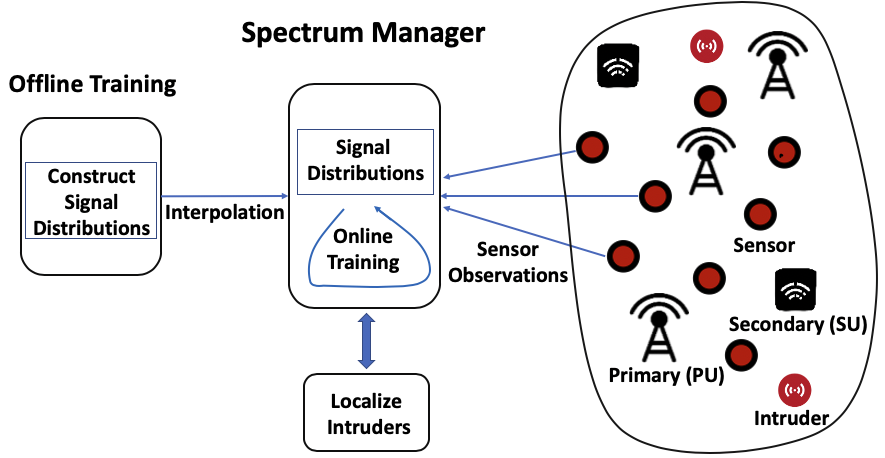
\includegraphics[width=0.95\textwidth]{chapters/ipsn/figures/architecture.png}
\caption{Overall approach to localize intruders in a shared spectrum system.} 
\label{fig:ipsn-illustration}
\end{figure}

The increasing affordability of the software-defined radio (SDR)
technologies makes the shared spectrums particularly prone to
unauthorized usage or security attacks. With easy access to SDR
devices~\cite{usrp,hackrf}, it is easy for selfish users to transmit data
on shared spectrum without any authorization and potentially causing
harmful interference to the incumbent users.  Such illegal spectrum
usage could also happen as a result of infiltration of computer virus
or malware on SDR devices.  As the fundamental objective behind such
shared spectrum paradigms is to maximize spectrum utilization, the
viability of such systems depends on the ability to effectively guard
the shared spectrum against unauthorized usage.  The current
mechanisms however to locate such unauthorized users (intruders) are
human-intensive and time-consuming, involving FCC enforcement bureau
which detects violations via complaints and manual
investigation~\cite{mobicom17-splot}. 
\eat{As explained below, an effective
technique should be able to accurately localize multiple simultaneous
intruders and even in the presence of dynamically changing set of
authorized users.}
Motivated by above, we seek for an effective
technique that is able to accurately localize multiple simultaneous
intruders and even in the presence of dynamically changing set of
authorized users. In the following, we begin with describing the multiple transmitter localization problem.


%%% Multi-tx and challenges.
\para{Multiple-Transmitter Localization (MTL).}  \eat{Localization of
unauthorized users in a shared spectrum system essentially boils down to localizing transmitters/intruders in a given area under a shared spectrum system.}
 The transmitter localization problem has been well-studied, but most of the focus has been on localizing a {\em single} intruder at a time. However, it is important to localize {\em multiple} transmitters {\em simultaneously} to effectively guard a shared spectrum
system. E.g., a malware or virus-based attachment could simultaneously cause many devices to violate spectrum allocation rules; spectrum
jamming attacks would typically involve multiple transmitters. More
importantly, a technique limited by localization of a single intruder
could then be easily circumvented by an offender by using multiple
devices.
The key challenge in solving the MTL problem comes from the fact that
the deployed sensor would receive only a sum of the signals from multiple transmitters, and separating the signals may be impossible.  In
addition, the other challenge that MTL in the context of shared
spectrum system poses is the presence of authorized users---e.g., the
incumbent users and the dynamic set of secondary users that have been
allocated spectrum by the manager. To the best our knowledge, no prior
localization work has considered the presence of authorized users.

%%%% SPLOT and shortcomings.
The state-of-the-art technique for the MTL problem is the recent
work~\cite{mobicom17-splot}, which essentially decomposes the MTL
problem to multiple single-transmitter localization problems based on
the sensors with the highest power readings in a
neighborhood. \eat{To the best of our knowledge, this is the only
  work that has addressed the MTL problem extensively, especially in
  the context of shared spectrum systems.} However, the technique has
a few shortcomings: (i) it implicitly assumes a propagation model, and
thus, may not work effectively in areas with complex propagation
characteristics, (ii) it is not effective in the case of transmitters
being located close-by, a key challenging scenario for MTL problem,
and (iii) most importantly, it can't be extended effectively to
incorporate background authorized users, a key requirement in the
context of shared spectrum systems. 
\eat{In our evaluation, we
  have compared our technique with theirs and one other approach.}
%%\blue{Our localization approach belongs to the fingerprinting~\cite{infocom00-radar} category.}

%%%%%%%W WHAT we DO.
\para{Our Approach.}  Transmitter localization is generally done based
on observations at deployed sensors. In particular, as in prior
works~\cite{mobicom17-splot,chakraborty2017specsense}, we assume a
crowdsourced sensing architecture wherein relatively low-cost spectrum
sensors are available for gathering signal strength in the form of
received power. Our approach is a hypothesis-driven Bayesian approach,
viz.\ {\em maximum a posteriori} (\map) approach, wherein each
hypothesis is a configuration (i.e.  a combination of $\langle
location, power \rangle$ pair) of the potential intruders, and the
goal is to determine the hypothesis that best explains the sensor
observations. This determination is done based on the distributions
(gathered during a training phase) of sensor observations for each
hypothesis.
%%%%%%%%%%%%
The \map approach is known to have optimal classification accuracy,
but (i) incurs prohibitive computation cost---exponential in number of
potential intruders---when applied to the \mtl problem, and (ii)
requires significant amount of training cost. The focus of our work is
to address these challenges, and design a viable \map-based approach.
%%%
In particular, using \map as a building block, we develop an optimized
approach that runs in polynomial time with minimized training cost.
We extend our technique to work in presence of authorized users by
incorporating online (real-time) training.

%%%%% MOTIVATION.
\softpara{Motivation for \map.}  Our motivation for using a \map-based
approach is multifold: First, with sufficient training data, \map is
known to deliver optimal classification accuracy for the MTL problem~\cite{map-optimal}.
Second, the \map approach doesn't assume any propagation model and
thus works for arbitrary signal propagation characteristics. Third, it
allows us to also estimate the intruder's transmit power, which can be
very useful in some applications, e.g., where the penalty is
proportional to the extent of violation. Last but not the least,
it naturally extends to being able to handle a presence of an evolving
set of authorized users.

\softpara{Training Cost and Optimization.}  The benefits of a \map-based
approach come at a cost: the \map framework requires prior training to
build probability distributions (PDs) of sensor observations for each
hypothesis. However, most of the training occurs offline, one-time,
and can be automated e.g.\ via drones or robots.  In our work, we
develop strategies to minimize the training cost; in particular, we
reduce the number of PDs to be constructed via a {\em novel interpolation
scheme} suited to our unique setting, and evaluate the impact of
reduced training on the localization accuracy.
%%%
We note that the online training to incorporate presence of authorized
users is needed only for the prevailing setting (of authorized
transmitters and deployed sensors) and hence incurs minimal cost
(see~\S\ref{sec:auth}).

\para{Overall Contributions.}  The goal of our work is to develop an
efficient technique for accurate localization of simultaneously
present multiple intruders in a shared spectrum system. The raw data are available at https://github.com/Wings-Lab/IPSN-2020-data. In this
context, we make the following four specific contributions. 
\begin{enumerate}
\item
Design an efficient localization algorithm (\ouralgo) for the MTL
problem, based on an optimal hypotheses-driven Bayesian approach. The
designed approach predicts both locations and transmit powers of the
intruders, and does not assume any propagation model and thus, works
for arbitrary signal propagation characteristics.

\item
Extend the designed algorithm (\ouralgoss) to localize effectively in
the presence of background authorized users, i.e., primaries with
possibly unknown parameters (e.g., location and transmit power) and an
evolving set of secondary users.

\item
Develop an effective interpolation scheme (\ildw) for our unique
setting to reduce the one-time training cost of our scheme, without
impacting the localization accuracy much.

\item
Evaluate our techniques via large-scale simulations as well as over
two developed testbeds (indoor and outdoor), and demonstrate the
effectiveness of our developed techniques and their superior
performance compared to the best-known techniques.
\end{enumerate}

%% We assume a crowdsourced architecture~\cite{}, wherein spectrum
%% sensing is delegated to independently deployed low-cost spectrum
%% sensors, such as rtl-sdr, who is merely over 20 dollars \cite{}.
%% Also there is a cloud-based spectrum manager~\cite{}, which 
%% orchestrates allocation of spectrum in such shared spectrum systems, 
%% based on available parameters and known channel conditions. 

%% The crowdsourcing spectrum sensor system scales well and realizes a
%% widespread and very cost-effective deployment.  Furthermore, it
%% facilitates the core spectrum management task we target at: guarding
%% the spectrum from unauthorized users.

%% Due to privacy, bandwith, and
%% cost concerns, it is impractical for the cheap sensors to send the
%% large raw signal I/Q samples to the cloud server.  Thus received
%% signal strength (RSS) is our choice of signal metrics.  So the sensors
%% process the raw signal I/Q samples locally and get RSS values, then
%% send the RSS values to the cloud.  Offloading the computation of
%% processing raw signal samples to the edge significantly decrease the
%% communication cost and enhance privacy.  T









% The best approach to date is \splot \cite{mobicom17-splot}, which utilized matrix inversion (essentially a variant of ridge regression) as a building block. However, it has an array of drawbacks. 
%% First and foremost, it is unable to localize two or more transmitters close by. 
%% The sensors' received signal is a phasor sum of the signals of both and \splot will report only one transmitter in the local maximum confined area.
%% Second, although it predicts location, it cannot predict the power of the transmitter. \splot is returning the coefficients of the ridge regression like function. 
%% The coefficients are correlated to the real power, but power is definitely not a function of those coefficients.
%% Third, the intrinsic mechanism of \splot assumes a propagation model.
%% They use a log normal model with an exponent of 2. However, the real environment may be more complicated than an ideal model, i.e. terrains can block and/or create multi-path reflection on the crowdsourced sensors.

%% The above three drawbacks comes from the settings of localizing only multiple illegal transmitters.
%% A fourth drawback will arise in the emerging shared spectrum system, where background transmissions from authorized users and potentially unauthorized offenders mixes together makes the proEvaluate our techniques via large-scale simulations as well as over
%two developed testbeds (indoor and outdoor), and demonstrate the
%effectiveness of our developed techniques and their superior
%performance compared to the best known techniques.blem harder by largely increasing the number of transmitters that need to be localized.
%% Multiple transmitter localization will hardly be perfect.
%% The more transmitters that need to localize, the less accuracy it gets.
%% For \splot, we see no good way of utilizing the information of authorized users to facilitate the localization of unauthorized offenders.
%% The way for \splot to work in a shared spectrum settings is to blindly localize all the transmitters and remove the known authorized users, then remains the unauthorized ones.
%% With this strategy, a smart spectrum offender can move close to an authorized user and safely transmit. 
%% \ble{In the mobicom-17 paper, they have a paragraph for dynamic localization, we might need to talk about it. It is a little related to our changing secondaries setting.}x

\section{Problem, Related Work, and Methodology}
\label{sec:ipsn-problem}

In this section, we describe our model of the shared spectrum systems,
formulate the \mtl problem, and discuss related work.  We also
describe the building block of our approach, viz., a hypothesis-driven
Bayesian localization approach (\map).

\para{Shared Spectrum System.} In a shared spectrum paradigm, the
spectrum is shared among licensed users (primary users, PUs) and
unlicensed users (secondary users, SUs) in such a way that the
transmission from secondaries does not interfere with that of the
primaries (or secondaries from a higher-tier, in case of a multi-tier
shared spectrum system~\cite{scte-isbe16-cbrs}). In some shared spectrum systems,
the location and transmit power of the primary users may be
unavailable, as is the case with military or navy radars in the CBRS
band~\cite{scte-isbe16-cbrs}.
%%%%%
Such sharing of spectrum is generally orchestrated by a centralized
entity called {\em spectrum manager}, such as a spectrum
database in TV white
space~\cite{sas-paper} or a central spectrum access system in
the CBRS 3.5GHz shared band~\cite{milind2015dyspan}. The spectrum
manager allocates spectrum to requesting secondaries (i.e., permission
to transmit up to a certain transmit power at their location) based on
their location, spectrum demand, configurations of the primaries, other
active secondaries, prevailing channel conditions, etc.
SwarmShare~\cite{jiangqi2021spectrum,jiangqi2023spectrum} is proposed to enable spectrum sharing
between the incumbent systems and the coexisting UAV networks in the 6GHz band.
Researchers have developed NeXT~\cite{jiangqi2022next,jiangqi2023next}, a software-defined wireless testbed, 
to support both traditional model-based control and new data-driven control techniques in wireless research.

\para{Authorized and Unauthorized Users.}
Secondary users that have been explicitly given permission to transmit
at their location are termed as {\em authorized users}; the primary
users are also considered as authorized users. Note that the set of
authorized users evolve over time, as more and more SUs are allocated
spectrum and as some SUs stop using the spectrum after a while. We can
assume that each SU is allocated spectrum for a certain duration of
time, after which it stops using the spectrum. 
%%%%%%%%%%%%
Other users that transmit without explicit permission (for that given
time) are referred to as {\em unauthorized users} or {\em intruders}.

\para{Problem Setting and Formal Definition.}  Consider a geographic
area with a shared spectrum. Without loss of generality, we assume a
single channel throughout this paper (multiple channels are handled
similarly). For localization of unauthorized users, we assume
available crowdsourced sensors that can observe the received signal in the
channel of interest, and compute (total) received signal strength
indicator (RSSI)\footnote{We do not use angle-of-arrival (AoA)
    measurements~\cite{aoa-multi} as they require additional and
    complex RF hardware.}. These sensors, being crowdsourced, may be at
  different locations at different times.  At any given instant, the
  shared spectrum area has some licensed primary users and some active
  secondary users; the PU configurations may not be known as can be
  the case for military users. The centralized spectrum manager is
  aware of the set of active SUs at any time, as each SU request is
  granted for a certain period of time.
%%%%
In addition to the authorized users, there may be a set of intruders
present in the area with each intruder in a certain ``configuration''
(see \S\ref{sec:map}).

The \mtl problem is to determine the set of intruders with their
configurations at each instant of time, based on the set of sensor
observations at that instant. See Figure \ref{fig:ipsn-illustration}. 
The basic \mtl problem assumes no other
transmissions (of authorized users) in the background.
%%%%%
The more general \mtl problem, where there may be an evolving set of
authorized users in the background, is referred to as the \mtlss
problem.  We address the \mtl problem in~\S\ref{sec:map-time}, and
then address the more general \mtlss problem in~\S\ref{sec:mtlss}.

%% Let $\theta_i = (l_i, p_i)$ denotes the configuration of location and
%% power of one transmitter, and $\boldsymbol{\theta_M} = \{\theta_1,
%% \theta_2, \cdots, \theta_M \}$ denotes the configurations of all
%% intruders. 
%% The problem is to predict $\boldsymbol{\theta_M}$ based on the observed received power
%% reported by sensor $\vx = \{x_1, x_2, \cdots, \}$.

\subsection{Related Work}
\label{sec:ipsn-related}

Localization of an intruder in a field using sensor observations has
been widely studied, but most of the works have focused on
localization of a single intruder~\cite{infocom18-spectrum,dutta2016see}.
%%%%%
In general, to localize multiple intruders, the main challenge comes
from the need to ``separate'' powers at the sensors~\cite{mobicom-30},
i.e., to divide the total received power into power received from
individual intruders. Blind source separation is a very challenging
problem; only very limited settings allow for known
techniques~\cite{freq-sig,ben-zhao} using sophisticated receivers. In
our context of hypotheses-driven approach, the challenge of source
separation manifests in terms of a large number of hypotheses, a
challenge addressed in~\S\ref{sec:map-time}.
%%%
We note that (indoor) localization of a
  device~\cite{infocom00-radar} based on signals received from multiple reference points (e.g, WiFi access
  points) is a quite different problem
  (see~\cite{zafari-19} for a recent survey), as the signals from
  reference points remain separate, and localization or tracking of multiple
  devices can be done independently.
  Recent works on multi-target localization/tracking are different in the way that targets are passive~\cite{ipsn19-multipassive, ipsn19-chorus, ipsn19-snaploc}, instead of active transmitters in this work.

In absence of blind separation methods, to the best of our knowledge,
only a few works have addressed multiple intruder(s) localization, and
none of these consider it in the presence of a dynamically changing
set of authorized transmitters. In particular,
(i)~\cite{mobicom17-splot} decomposes the multi-transmitter
localization problem to multiple single-transmitter localization
problems based on the sensors with highest of readings in a
neighbohood, (ii)~\cite{clustering} works by clustering the sensors
with readings above a certain threshold and then localizing intruders
at the centers of these clusters, (iii)~\cite{Quasi-EM} uses an
EM-based approach.
%%%
The techniques of~\cite{mobicom17-splot,Quasi-EM} assume a propagation
model, while that of~\cite{clustering,Quasi-EM} require a priori
knowledge of the number of intruders present.  We have compared our
approach with~\cite{mobicom17-splot,clustering} in \S\ref{sec:eval},
while~\cite{Quasi-EM} has high computational cost and has also been
shown to be inferior in performance
to~\cite{mobicom17-splot,clustering} even for a small number of
intruders. Other related works include
  (i)~\cite{multi-tx-dyspan-19} that addresses the challenge of
  handling time-skewed sensors observations in the MTL problem, and
  (ii)~\cite{info-20} that addresses the sensor selection optimization
  problem for our proposed hypotheses-based localization approach.
  
%%%%%
%\blue{Other related works include:~\cite{mobicom-22} where sensors are
%  on mobile and controlled robots,~\cite{mobi-25} focusses on spectrum
%  allocation via spectrum hole detection in presence of background 
%  transmitters.} \red{HG: Remove this sentence?}

%% Online selection of sensors: ipsn-04, .... latency vs. energy .. since,
%% latency is equally critical, ... we dont want to run it for every intruder ... 
%% Similarly,
%% \cite{krause2008near} shows that minimizing uncertainty in a gaussian
%% process is submodular, and thus greedy selection provides a bounded
%% solution to the optimal.

%% Multiple studies have studied sensor selection to maximize the
%% accuracy of detection of some event \cite{rowaihy2007survey}.

%% For
%% example, \cite{joshi2009sensor} provides a heuristic for sensor
%% selection by forming a convex optimization problem.  However, it uses
%% a different metric to measure the accuracy of detection.
%% %%%%
%% Other studies, such as
%% \cite{shamaiah2010greedy} and \cite{bian2006utility} have proposed
%% leveraging submodularity to select sensors.  

%% There are also studies in the active learning literature that focus on
%% online selection.  For example, \cite{yuxin-when} limits the mutual
%% information while selecting the minimum possible number of sensors.
%% \cite{krause2012near} shows that mutual information in sensor
%% selection is submodular in the absence of noise and propose a
%% probabilistic greedy algorithm by leveraging it.
%% \cite{golovin2011adaptive} proposes the concept of adaptive
%% submodularity that generalizes the greedy approximation to online
%% selection. Our online selection algorithm builds upon these studies to
%% limit the number of sensors while maximizing the mutual information.
%% However, in the presence of noise, mutual information is not adaptive
%% submodular in nature.  Thus, our work modifies the algorithm discussed
%% in \cite{yuxin-when} to make it suitable for our use case.


\subsection{\map: Bayesian Approach for Localization}
\label{sec:map}

We localize intruders based on observations from a set of
sensors. Each sensor communicates its observation to a centralized
entity, the spectrum manager, which runs an appropriate
localization algorithm to localize the intruders.
%%%%
In particular, we use a hypotheses-driven Bayesian approach, as
described below, where intruders are localized by determining the
most likely prevailing hypothesis; this is done based on joint
probability distributions of the sensors' observations (constructed
during a priori training). Below, we formalize the above concepts, and
the basic localization approach.

\para{Observation; Observation Vector.} Throughout this
paper, we use the term {\em observation} at an individual sensor to
mean the received power over a time window of certain duration, in the
frequency channel of interest (we assume only one channel). In
particular, received power is computed from the FFT of the I/Q samples
in the time window~\cite{arani2018}. We use the term {\em observation
  vector} \vx to denote a vector of observations from a given set of
distributed sensors, with each vector dimension corresponding to a
unique sensor.
%%%%%%%%
%% We assume a Gaussian distribution $N (\mu, \sigma^2)$ for each
%% observation, where mean implies the average power the receiver
%% receive, and standard deviation will represent the noise, shadowing,
%% and multi-path fading.

\begin{wrapfigure}{r}{2in}
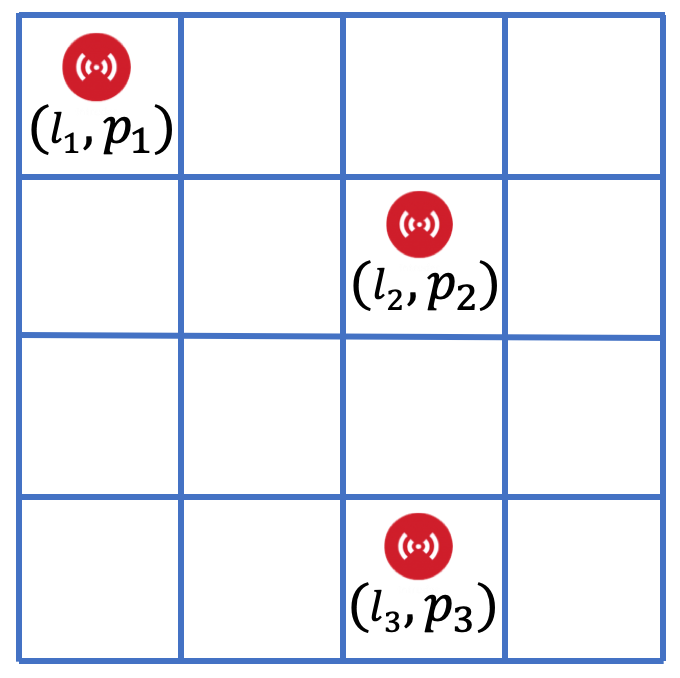
\includegraphics[width=2in]{chapters/ipsn/figures/hypothesis.png}
\caption{Illustration of a hypothesis formed of three transmitters.}
\label{fig:hypothesis-grid}
\end{wrapfigure}
\para{Hypotheses.} Let \hz, \ho, $\ldots,$ \hM be the set of all
hypotheses, where each hypothesis \hj represents a ``configuration''
of potential intruders. In this chapter, we largely assume an
  intruder's configuration to be comprised of just its location and
  transmit power, but the concept of configuration is quite general
  and could include any attributes (e.g., height, antenna direction,
  etc.) that affect how its transmitted signal is received at other
  locations. Moreover, for simplicity, we assume that each intruder
  transmits at a fixed power (which may be different for different
  intruders). Thus, in our context, a configuration is simply the set
of (location, transmit power) pairs of potential intruders. We
assume a bounded number of intruders. We use \hz to represent the
hypothesis with no intruders. See Figure~\ref{fig:hypothesis-grid}.

%%%%%%%
If there is only one intruder, then each hypothesis represents the
location and transmit power combination of the intruder, and
determining the hypothesis is equivalent to localizing the intruder
and estimating its power. If we allow multiple intruders at a time,
the number of possible hypotheses can be exponential in the number of
intruders; we will address this challenge in
\S\ref{sec:map-time}.

\softpara{Inputs.} For a given set of sensors deployed over an area, we
assume the following available inputs, obtained via a priori training,
data gathering and/or analysis:
\begin{itemize}
\item
Prior probabilities of the hypotheses, i.e. $P(H_i)$, for each
hypothesis $H_i$. Prior probabilities come from known knowledge about
the area, intruder's behavior, etc., and can be assumed to be uniform in
absence of better knowledge.

\item
Joint probability distribution (JPD) of sensors' observations for each
hypothesis. More formally, for each hypothesis $H_j$, we assume
$P(\vx|H_j)$ to be known for each observation $\vx$ for the set of
deployed sensors.  The JPDs can be obtained from prior training, a
combination of training and interpolation (\S\ref{sec:inter}), or
even by assuming a propagation model to remove the training
cost completely.
\end{itemize}

\para{Maximum a Posteriori (\mll) Localization Algorithm.}  We use
Bayes rule to compute the likelihood probability of each hypothesis,
from a given observation vector $\vx$:
\begin{equation}
  P(H_i | \vx) = \frac{P(\vx| H_i)P(H_i)}{\sum_{j=0}^m P(\vx|H_j)P(H_j)}
  \label{eqn:bayes}
\end{equation}
We select the hypothesis that has the highest probability, for given
observations of a set of sensors. That is, the \mll Algorithm returns
the hypotheses based on the following equation:
\begin{equation}
  \arg \max_{i=0}^m P(H_i | \vx)
  \label{eqn:map}
\end{equation}
The above \mll algorithm to determine the prevailing hypothesis is
known to be {\em optimal}~\cite{map-optimal}, i.e., it yields the minimum
probability of (misclassification) error. The above hypothesis-based
approach to localization works for arbitrary signal propagation
characteristics, and in particular, obviates the need to assume a
propagation model. However, the above \mll algorithm does incur a {\em
  one-time} training cost to construct the JPDs.




\section{{\texorpdfstring{\ouralgo}: Optimizing \mll for MTL}}
\label{sec:map-time}

The \map algorithm of \S\ref{sec:map} can be directly applied to
localize multiple intruders with optimal localization accuracy.
However, \map incurs prohibitive computational costs, especially for a
large number of potential intruders.  In particular, note that if
there are $L$ potential locations, up to $T$ potential intruders, and
$W$ possible discrete transmit-power levels, then the
hypotheses-driven \map algorithm needs to consider $(LW)^T$
hypotheses---making its runtime complexity exponential in the number of
potential intruders, and thus, making it impractical to localize
even a moderate number of intruders present simultaneously.  In
addition, \mll also incurs a high training cost. In the following
subsections, we develop an optimized algorithm called \ouralgo based
on \map but with significantly improved computational and
training cost.
%%%%%
We start with optimizing the computation cost in \S\ref{sec:time}. In the following
  subsection \S\ref{sec:ipsn-power}, we derive a closed-form expression
  to efficiently estimate the intruder's power in the {\em continuous}
  domain.  Finally, we discuss optimizing the training cost via a
  novel interpolation scheme \ildw.

%% Next, we use this result to design a computationally
%% efficient algorithm in the following section
%% 2) optimizing the \map algorithm in a way that
%% minimizes the subarea where ``simultaneous'' localization of multiple
%% intruders needs to be considered (the source of exponential
%% complexity).  The former cancels $W$ in the base and the later reduces
%% $L$ in the base.

%\subsection{Intruder Power Estimation in the Continuous Domain}
\label{sec:ipsn-power}

In this subsection, we derive a {\em closed-form} expression to estimate an
intruder's power in the continuous domain, for the special case of
single intruder and Gaussian probability
distributions~\cite{gauss}. The derived result essentially removes the
assumption of discrete power levels, and reduces the number of
hypotheses to consider by a factor of $W$. We use
this result within Procedure~1 of the previous subsection to further
optimize its time complexity and performance.

\para{Estimating Intruder Power, Given a Location.}  Consider the
special case of a single intruder in an area. In this case, each
hypothesis can be represented as \hlp, for each location $l$ and power
$p$ of the potential intruder. Let us focus on a particular location
$\lstar$ and the corresponding hypotheses \hLp. 
%%%%%
For a given observation vector \vx, we wish to estimate the power $P$
that corresponds to the hypothesis with maximum likelihood among the
hypotheses \hLp.
$$P = \arg max_p P(\hLp | \vx)$$
%%%%
The value $P$ can be computed by computing $P(\hLp | \vx)$ for
each $p$, but our goal is to derive a closed-form expression for $P$
from the given JPDs; such an expression yields power estimate in
continuous domain without computing $P(\hLp | \vx)$ for each possible
discrete $p$.

For each sensor (location) $j$, let $\pd(\vx_j | \hLP)$ represent the
probability distribution (PD) of $j$'s observations $\vx_j$ when the
intruder is at \lstar transmitting with power \pstar, the power used
at training.
%%%%%%
For a fixed \lstar and \pstar, the set of PDs $\pd(\vx_j | \hLP)$ are
equivalent to the JPDs defined in \S\ref{sec:ipsn-problem} under the
assumption of conditional independence\footnote{PD $\pd(\vx_j |
  \hLp)$ can be computed $\pd(\vx_j | \hLP)$ for any $p$, as the
  path-loss can be assumed to be independent of the transmit power,
  and JPD $\pd(\vx | \hLp)$ can be computed as product of PDs
  $\pd(\vx_j | \hLp)$ due to the conditional independence assumption.}.
%%%%%%%
%%%%%%%%
Let us assume that the above PDs are Gaussian
distributions~\cite{gauss}, and thus, can be represented as $\pd(\vx_j
| \hLP) = N(\mu_j, \sigma_j^2)$ for a given $\lstar$ and $\pstar$.
%%%%%%%%%%%%%
In the above setting, the power value $P$ that maximizes $P(\hLp | \vx)$
can actually be derived as a closed-form expression; we state the result
formally in the below lemma. 
\begin{lemma-wo-prf}
  Consider the special case of a single intruder in an area.  For a
  specific location $\lstar$ and power $\pstar$ (the only power used
  during training), let $\pd(\vx_j | \hLP)$ represent the PDs of the
  sensor observations at location $j$. Now, given the above PDs for
  various $j$ and an observation vector $\vx$, the power value
  $P = \arg max_p P(\hLp | \vx)$ is   given by: 
  $$\pstar + \frac{\sum_{j=1}^{S} \frac{\gamma}{\sigma_j^2}(x_j - \mu_j)}{\sum_{j=1}^{S} \frac{\gamma}{\sigma_j^2}},$$
  where $\gamma = \prod_{j=1}^{S} \sigma_j^2$ and S equals the number of sensors in the neighborhood of  $\ \lstar$.
  \label{lem:p}
\end{lemma-wo-prf}
The proof is in Appendix~\ref{appen:ipsn}. 
Here, we give its intuition based on a special case. 
Consider the special case wherein each $\sigma_j$ is 1 for all
$j$. In this special case, the Lemma's equation reduces to $P = \pstar
+ \frac{\sum_{j=1}^{S}(x_j - \mu_j)}{|S|}$, which implies that if each
observation $x_j$ is $c$ more than its mean $\mu_j$ then $P$ is also
$c$ more than $\pstar$. We note that the above result does {\em not}
extend to the case of multiple intruders. In short, the proof is a process of solving maximum likelihood estimation and multiple intruders introduce transcendental functions, thus cannot derive a closed-form solution.

\para{Use of Lemma~\ref{lem:p} in \ouralgo.} \eat{First, we note that,
  for the special case of a single intruder, the result of
  Lemma~\ref{lem:p} essentially allows us to determine continuous
  power value of the intruder while also reducing the overall
  computational complexity of the optimal \mll algorithm by a factor
  of $W$, the number of discrete power levels.}  For localization of
multiple intruders, Lemma~\ref{lem:p} can only be used in Procedure~1
of \S\ref{sec:time}, due to its assumption of a single intruder. In
particular, we can Procedure~1 of \S\ref{sec:time} as follows.
\begin{itemize}
\item
We replace \Rp by $R$, the maximum transmission radius.
  
\item
For each location $l$, using Lemma~\ref{lem:p}, we first compute the
power $p(l)$ such that the hypothesis \hlpl has the most likelihood
(among the hypotheses at $l$) using the observations from sensors
within a radius of $R$.
\item
Then, in the rest of the procedure, we only consider the (location,
power) pairs of the type $(l, p(l))$ for any $l$.
\end{itemize}
The rest of the Procedure~1 remains unchanged. The above change has two
benefits. First, the powers predicted in Procedure~1 are now
continuous rather than discrete. Second, the above removes the factor
of $W$ from the time complexity of \ouralgo and reduces it to
$O(LG_R\log(G_R) + G_R(G_R)^T)$ which becomes $O(L)$ if we consider
$G_R$ and $T$ to be relatively small constants.


\subsection{Optimizing Computation Time}
\label{sec:time}

\para{Basic Idea.}  Note that the \mll's exponential time complexity
is due to the exponential number of {\em combinations} of locations
and/or powers of the potential intruders. To motivate our proposed
optimized approach, consider a simple example of 2 intruders with
fixed power $p$ in a large area. Assume that the ``transmission
radius'' $r$ for power $p$ is much smaller than the area; we define
the {\em transmission radius} as the range till which the received
signal is more than a certain noise floor.
%%%%
The key observation is that if the intruders are far away (isolated)
from each other (specifically, more than $2r$ distance away), then
they could be localized independently. If the intruders are closer,
then there is a need to separate aggregated signal at some of the
sensors and hence we must apply the standard \mll algorithm {\em
  within that ``subarea''}; however, since each such subarea is small
(a disk of $2r$ radius around each possible location), the computation
time is reduced significantly. However, since we do not a priori know
the configurations of intruders, we need to consider appropriate
possibilities.

In essence, our optimized approach is a divide-and-conquer approach,
consisting of a sequence of two procedures each of which is executed
iteratively. The first procedure focuses on localizing ``isolated''
intruders (if any) independently, while the second procedure localizes
the remaining intruders---by considering all possible subareas as
suggested above. The challenge lies in modifying the \mll algorithm
for each iteration of the above procedures---as the hypotheses to
consider across iterations of the procedures are not disjoint. We now
describe each of the procedures.

\para{Procedure 1. Localize Isolated Intruders.}  Informally, in this
procedure, we localize intruders that are sufficiently separated from
other intruders. In other words, we localize intruders $x$ that are
surrounded by sensors that receive most of their received power from
$x$. More formally, we localize an intruder $x$ at location $l$ if (i)
$l$'s ``neighborhood'' has at least 3 sensors that receive most of
their power from $x$, and (ii) there are no other intruders in the
``vicinity'' of $l$. In essence, we iterate over all locations $l$,
and localize an intruder at $l$ if the above conditions are satisfied
with high enough probability, based on the readings of sensors around
$l$.
%%%%%
The precise definition of neighborhood above must depend on $x$'s
transmission radius which depends on its transmit power; however, as
$x$'s transmit power is unknown, we iterate over smaller and smaller
neighborhoods.

We now formally describe the procedure.  Let \Rp denote the
transmission radius for a transmit power of $p$. Let $R$ denote the
maximum transmission radius, i.e., $$\max_p \Rp.$$ In the below
description, we use a fractional value $f$ to define a neighborhood
and vicinity size. We start $f$ equal to 1, use a disk of radius
$f\Rp$ as a neighborhood and $R + f\Rp$ as the vicinity, and iterate
over the procedure for reduced values of $f$.
\begin{packedalpha}
	\item
	Let $f$ = 1.
	
	\item
	For each location and power pair $(l,p)$, compute $P(\hlp |
        \vxlp)$ using a form of Equation~\ref{eqn:bayes} over
        appropriate JPDs. Here:
        \begin{itemize}
          \item
         \hlp represents the hypothesis that an intruder is at
         location $l$ and using $p$ transmit power. We also implicitly
         assume that there is no other intruder present within a
         distance of $R + f\Rp$ from $l$; this ensures that the
         observations in $\vxlp$ are only due to the intruder at $l$.
         See Figure ~\ref{fig:mmap}.
         
       \item
         $\vxlp$ represents the observation vector for all sensors,
         but the sensors that are within a radius of $f\Rp$ around
         $l$ use an observation of ``residual'' received powers, as
         defined below, while the remaining sensors (outside the
         radius of $f\Rp$ around $l$) use an observation of the
         ``noise floor'' (in essence, we are ``zeroing'' the
         observations of the far-away sensors). See Figure~\ref{fig:mmap}.
         \end{itemize}
	
	\item
	Denote $(l,p)$ pairs that have $P(\hlp | \vxlp)$ higher than a
        certain threshold as {\em peaks}. If a location $l$ is a peak
        and there are no other peaks within a distance of $R + f\Rp$,
        then {\bf localize an intruder at $l$ with transmit power
          $p$.}

      \item
	For each sensor $s$, define its {\em residual received power}
          (RRP) as the total received power reduced by the sum of
        mean powers received from already localized intruders; the
        desired mean values are available from the given
        JPDs.
	
	\item
	Reduce $f$ and go back to step \#2 above, unless no new
        intruders were localized in (c) above. In our experiments, we
        used $f = 1, 1/2, 1/4$ and $1/8$.
\end{packedalpha}

\begin{figure}
	\centering
	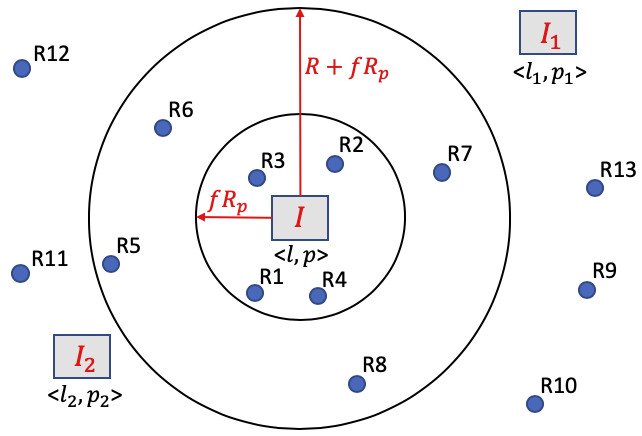
\includegraphics[width=0.7\textwidth]{chapters/ipsn/figures/mmap.png}
	\caption{Illustration of Hypothesis \hlp in Step (b) of
          Procedure~1. Here, the intruder $I$ at location $l$ is
          transmitting at power $p$, with no other intruder within a
          distance of $R + f\Rp$ from $I$. The observation vector
          $\vxlp$ consists of residual received powers from $R1$ to
          $R4$, and ``noise floor'' from the remaining sensors.}
	\label{fig:mmap}
\end{figure}

The above procedure is partly inspired by the recent localization
work~\cite{clustering}. However, instead of discarding sensors based
on their individual power and clustering the rest as
in~\cite{clustering}, we ``discard'' sensors based on their
neighborhood readings (i.e., likelihood $P(\vx| H_i)$ values) and then
``cluster'' the remaining sensors. Also, we ``cluster'' iteratively,
for smaller and smaller neighborhoods.

%% Our above procedure is partially inspired by the recent localization
%% work~\cite{clustering}, which discards sensors that receive power
%% below a certain threshold, clusters the remaining sensors, and then
%% place an intruder in each cluster. In effect, we ``discard'' a sensor
%% $s$ based on information from $s$'s neighborhood (i.e., likelihood P()
%% values) rather than $s$'s individual power as in~\cite{clustering}.
%% Also, as an improvement over~\cite{clustering}, we ``cluster''
%% iteratively, a small number of times. 
%%%%
%% Another saliant aspect of the above procedure is that we localize
%% these separated intruders based on the likelihood $P()$ function which
%% is defined for {\em each} location; in contrast, past approaches such
%% as~\cite{mobicom_utah, clustering} have localized such separated
%% intruders {\em directly} based on sensor obversations which can be
%% sparse for less dense sensor deployents and thus, yield more
%% noisy/inaccurate results.

\para{Procedure 2. Localize Intruders Situated Close-By.}  Once we
have localized separated intruders as above, we now localize the remaining
intruders, if any, by applying the general \map algorithm
independently over ``subareas'' that still have some sensors with
high-enough RRP (residual received power), but no intruder localized
in the ``vicinity.'' Formally, the procedure is as follows. Let $T$ be
the maximum number of intruders allowed within a disk of radius $R$,
the maximum transmission radius.

\begin{packedalpha}
 \item
Let $s$ be the sensor with the highest RRP; if $s$'s RRP is below a
certain threshold (tantamount to noise), then quit.

\item
For $t$ = 2 to $T$: Use \map (from \S\ref{sec:map}) to try to localize
$t$ transmitters within a disk of radius $R$ around $s$, using
observations of sensors within a radius of $2R$ from $s$. We use a
certain threshold for a posterior probability, in a similar way as for
Procedure~1.

\item
Update RRP of each sensor, and go to step (a) above.
\end{packedalpha}
%%%%%%%%%%%

\para{Time Complexity.} The worst-case time complexity of the first procedure is \\
$O(LWG_R\log(G_R))$, where $L$ and $W$ are the number
of potential locations (total grid cells) and transmit power levels
respectively, and $G_R$ is the maximum number of grid cells within a
transmission range of an intruder.
%%%
Here, the first term $O(LWG_R)$ is the time to compute the likelihood
values in each iteration, since the number of sensors involved in each
computation is at most $G_R$. Note that the number of iterations is
bounded by $\log(G_R)$, as $f$ is reduced by a constant multiplicative
factor.
%%%
The worst-case time complexity of the second procedure is
$O(G_R(G_R)^T)$ where $T$ is the maximum number of intruders
allowed/possible in a transmission region (i.e., a circle of radius at
most $R$).
Thus, the overall time complexity of the above localization algorithm
is $O(L.W.G_R.\log(G_R) + G_R.(G_R)^T)$.
%%%%
Generally, we would expect $T$ to be a small constant, as more than 3
intruders in a $R$-radius region with a $R$ transmission range would
interfere with each other. If we also consider $G_R$ as a small
constant, the overall time complexity can be considered to be
$O(L.W)$.  In the following subsection, we further reduce the time
complexity by removing the factor of $W$.

\subsection{Intruder Power Estimation in the Continuous Domain}
\label{sec:ipsn-power}

In this subsection, we derive a {\em closed-form} expression to estimate an
intruder's power in the continuous domain, for the special case of
single intruder and Gaussian probability
distributions~\cite{gauss}. The derived result essentially removes the
assumption of discrete power levels, and reduces the number of
hypotheses to consider by a factor of $W$. We use
this result within Procedure~1 of the previous subsection to further
optimize its time complexity and performance.

\para{Estimating Intruder Power, Given a Location.}  Consider the
special case of a single intruder in an area. In this case, each
hypothesis can be represented as \hlp, for each location $l$ and power
$p$ of the potential intruder. Let us focus on a particular location
$\lstar$ and the corresponding hypotheses \hLp. 
%%%%%
For a given observation vector \vx, we wish to estimate the power $P$
that corresponds to the hypothesis with maximum likelihood among the
hypotheses \hLp.
$$P = \arg max_p P(\hLp | \vx)$$
%%%%
The value $P$ can be computed by computing $P(\hLp | \vx)$ for
each $p$, but our goal is to derive a closed-form expression for $P$
from the given JPDs; such an expression yields power estimate in
continuous domain without computing $P(\hLp | \vx)$ for each possible
discrete $p$.

For each sensor (location) $j$, let $\pd(\vx_j | \hLP)$ represent the
probability distribution (PD) of $j$'s observations $\vx_j$ when the
intruder is at \lstar transmitting with power \pstar, the power used
at training.
%%%%%%
For a fixed \lstar and \pstar, the set of PDs $\pd(\vx_j | \hLP)$ are
equivalent to the JPDs defined in \S\ref{sec:ipsn-problem} under the
assumption of conditional independence\footnote{PD $\pd(\vx_j |
  \hLp)$ can be computed $\pd(\vx_j | \hLP)$ for any $p$, as the
  path-loss can be assumed to be independent of the transmit power,
  and JPD $\pd(\vx | \hLp)$ can be computed as product of PDs
  $\pd(\vx_j | \hLp)$ due to the conditional independence assumption.}.
%%%%%%%
%%%%%%%%
Let us assume that the above PDs are Gaussian
distributions~\cite{gauss}, and thus, can be represented as $\pd(\vx_j
| \hLP) = N(\mu_j, \sigma_j^2)$ for a given $\lstar$ and $\pstar$.
%%%%%%%%%%%%%
In the above setting, the power value $P$ that maximizes $P(\hLp | \vx)$
can actually be derived as a closed-form expression; we state the result
formally in the below lemma. 
\begin{lemma-wo-prf}
  Consider the special case of a single intruder in an area.  For a
  specific location $\lstar$ and power $\pstar$ (the only power used
  during training), let $\pd(\vx_j | \hLP)$ represent the PDs of the
  sensor observations at location $j$. Now, given the above PDs for
  various $j$ and an observation vector $\vx$, the power value
  $P = \arg max_p P(\hLp | \vx)$ is   given by: 
  $$\pstar + \frac{\sum_{j=1}^{S} \frac{\gamma}{\sigma_j^2}(x_j - \mu_j)}{\sum_{j=1}^{S} \frac{\gamma}{\sigma_j^2}},$$
  where $\gamma = \prod_{j=1}^{S} \sigma_j^2$ and S equals the number of sensors in the neighborhood of  $\ \lstar$.
  \label{lem:p}
\end{lemma-wo-prf}
The proof is in Appendix~\ref{appen:ipsn}. 
Here, we give its intuition based on a special case. 
Consider the special case wherein each $\sigma_j$ is 1 for all
$j$. In this special case, the Lemma's equation reduces to $P = \pstar
+ \frac{\sum_{j=1}^{S}(x_j - \mu_j)}{|S|}$, which implies that if each
observation $x_j$ is $c$ more than its mean $\mu_j$ then $P$ is also
$c$ more than $\pstar$. We note that the above result does {\em not}
extend to the case of multiple intruders. In short, the proof is a process of solving maximum likelihood estimation and multiple intruders introduce transcendental functions, thus cannot derive a closed-form solution.

\para{Use of Lemma~\ref{lem:p} in \ouralgo.} \eat{First, we note that,
  for the special case of a single intruder, the result of
  Lemma~\ref{lem:p} essentially allows us to determine continuous
  power value of the intruder while also reducing the overall
  computational complexity of the optimal \mll algorithm by a factor
  of $W$, the number of discrete power levels.}  For localization of
multiple intruders, Lemma~\ref{lem:p} can only be used in Procedure~1
of \S\ref{sec:time}, due to its assumption of a single intruder. In
particular, we can Procedure~1 of \S\ref{sec:time} as follows.
\begin{itemize}
\item
We replace \Rp by $R$, the maximum transmission radius.
  
\item
For each location $l$, using Lemma~\ref{lem:p}, we first compute the
power $p(l)$ such that the hypothesis \hlpl has the most likelihood
(among the hypotheses at $l$) using the observations from sensors
within a radius of $R$.
\item
Then, in the rest of the procedure, we only consider the (location,
power) pairs of the type $(l, p(l))$ for any $l$.
\end{itemize}
The rest of the Procedure~1 remains unchanged. The above change has two
benefits. First, the powers predicted in Procedure~1 are now
continuous rather than discrete. Second, the above removes the factor
of $W$ from the time complexity of \ouralgo and reduces it to
$O(LG_R\log(G_R) + G_R(G_R)^T)$ which becomes $O(L)$ if we consider
$G_R$ and $T$ to be relatively small constants.


\subsection{\ildw: Optimizing Training Cost}
\label{sec:inter}

As in supervised machine learning algorithms, our Bayesian approach
also needs training data.  We use the term
\emph{training} to denote the process of collecting data and building
up the JPDs for the hypotheses. Note that this training phase is done
only one-time,\footnote{JPDs depend on the channel state and
    hence, must be updated periodically to account for any changes in
    the environment (e.g., terrain, buildings, etc.); however, such
    environment changes are infrequent. Also, note that the
    online-training of~\S\ref{sec:auth} is done repeatedly, but only
    for specific sensors and authorized users, and thus incurs minimal
    cost. See ~\cite{mobicom19-bigspec} for spectrum sensing in both spatial and temporal domains. }
and hence, a certain cost is acceptable. The training cost
incurred during such data gathering depends greatly on the exact
mechanism used for such purposes, e.g., drones with appropriate routes
can be used to gather such data~\cite{robot-ref}.  In general, the
cost of training would depend on the number of JPDs that need to be
constructed, with the cost reduced with a reduction in the number of
JPDs needed. In this subsection, we design effective {\em interpolation}
schemes that are useful in reducing the number of JPDs gathered which
in turn will reduce the overall training cost. Note that reduction in
JPDs constructed from raw data is bound to negatively impact the
accuracy---we will evaluate this trade-off in our evaluations and show
that impact on accuracy is minimal even with a significant reduction in
training cost.

\para{Probability Distributions.}  First, we note that making the
following reasonable assumptions and observations can greatly reduce
the number of JPDs/PDs to be constructed.
\begin{itemize}
  \item
If we assume conditional independence of sensor observations, then
JPDs can be computed from independently constructed probability
distributions (PDs) of received powers at {\em individual sensors}.

\item
  Since received power at a sensor location $x$ due to multiple
  transmitters is merely a sum of received powers~\cite{rappaport-2001,mobicom17-splot} due to individual
  transmitters, we can compute PD at $x$ for a particular hypothesis
  involving a set $S$ of intruders from PDs due to each individual
  intruder in $S$.

\item
  Lastly, we need to only construct a PD for one transmit power for
  each transmitter and sensor location pair, since path loss is
  independent of transmit power.
\end{itemize}
Based on the above observations, if there are $L$ discrete locations
in an area for sensors or intruders, then a \mll-based approach
requires $L^2$ PDs. Below, we propose to minimize the number of PDs to
be constructed via data gathering/training, by estimating the
remaining unconstructed PDs via interpolation.


\begin{figure}
  \center
  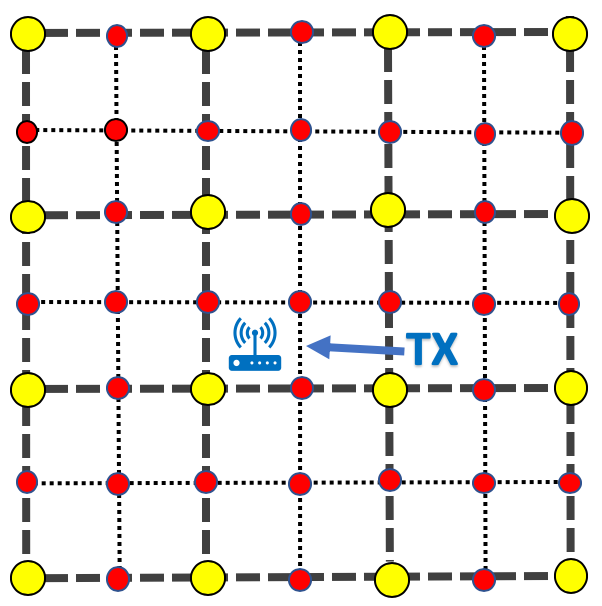
\includegraphics[width=0.45\textwidth]{chapters/ipsn/figures/multi-granular.png}
  \caption{Training for PDs at coarse-grained locations (yellow bigger
          dots), while estimating PDs using interpolation at the remaining
          fine-grained locations (red smaller dots).}
  \label{fig:path-loss}
\end{figure}

\para{Minimizing Training Cost with \ildw.} Consider a particular
location \lstar of a potential intruder. Our eventual goal is to
compute the PD for each of the $L$ possible sensor locations for this
location \lstar of a potential intruder; a PD may be computed either
by constructing it directly from gathered sensor observations or by
estimation via interpolation from the constructed PDs. In particular,
for effective interpolation, we construct PDs at coarser-grid sensor
locations and estimate via interpolation the PDs at the remaining
finer-grid locations. See Figure~\ref{fig:path-loss}. The exact
coarseness at which the PDs are constructed is determined by the
accuracy of the interpolation scheme for a given area and/or the
impact on localization accuracy due to estimated PDs. Below, we
describe the interpolation scheme that we use for our purposes.


\begin{figure}
  \begin{subfigure}[t]{0.9\textwidth}
    \centering
    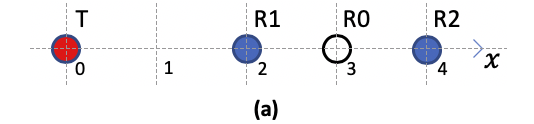
\includegraphics[width=0.5\textwidth]{chapters/ipsn/figures/interpolate.png}
  \end{subfigure}
  \qquad
  \newline
  \begin{subfigure}[t]{\textwidth}
    \centering
    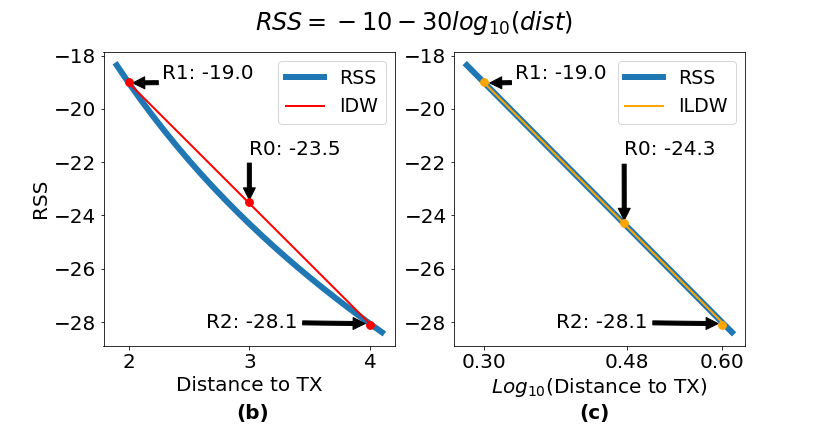
\includegraphics[width=0.8\textwidth]{chapters/ipsn/figures/ildw.png}
  \end{subfigure}
  \caption{Illustration of \ildw vs.\ IDW.
  (a) Transmitter (T), points with known (R1 and R2) and unknown (R0) received signal strength (RSS) values.
  (b) Log-normal RSS function (= -10 - 30$\log_{10}({\rm distance}))$
  plotted for varying distance from the transmitter $T$, along
  with IDW-estimated RSS value at a point between R1 and R2.
  (c) Log-normal RSS function and ILDW-estimated RSS value at
  a point between R1 and R2, plotted on a logarithmic distance
  scale.}
  \label{fig:ildw}
\end{figure}

\softpara{\ildw Interpolation Scheme.} Consider a fixed transmitter
location \lstar, and let us assume locations $\lo, \rt, \cdots, \lm$ for
which we know the path loss from \lstar. Now, consider a new point \lz
for which we wish to estimate the path-loss from \lstar.
%%%%%%%%%%%%
This is a traditional interpolation problem and well-known schemes
such as inverse distance weighting (IDW), Ordinary Kriging (OK), k-NN,
etc. have been evaluated even in the special context of signal
strength or received power~\cite{chakraborty2017specsense}.
%%%%
However, our specific context has a unique element. We
{\em know} the location \lstar of the transmitter from which the
path-loss is being estimated---as we are in the training phase wherein
we are gathering observations with the transmitter at \lstar.
\eat{ (ii) Second,
the points with known values viz.\ $\lo, \rt, \cdots, \lm$ are not
arbitrary or random points, but can be chosen to facilitate accurate
estimation (e.g., in our scheme, as mentioned above, we have chosen
them to be at coarser {\em uniform} grid locations).}
%%%%%%%%
In light of the above unique element of our setting, and the observation of wireless signal characteristics, we use a custom
interpolation technique which is a nontrivial modification of the IDW
scheme, called {\em inverse log-distance weighting} (\ildw). The traditional
IDW interpolation scheme estimates the
path loss at \lz by taking a weighted average of the path losses at
$\lo, \rt, \cdots, \lm$, with the weight being the inverse of the
distance from \lz. 
%%%%%

In our proposed \ildw scheme, we still estimate the path loss at \lz as
a weighted average of values at \li's, but assign weights differently.
In particular, we assign the weight for the point \li as the inverse
of the ``distance'' between \lz and \li in the domain where each point
is represented merely by its logarithmic distance from \lstar, the known
transmitter's location---i.e., each point $\li$ is mapped to a point
$\log d(\li, \lstar)$ on a line. This mapping is motivated by the
expectation that the actual path loss would be somewhat similar to the
log-distance path loss.
%%%%%%%
Thus, the weight for the point $\li$ is assigned to be
$$w_i = \frac{1}{|\log d(\li, \lstar) - \log d(\lz, \lstar)|},$$ where $d()$ is the
Euclidean distance function and the path loss at \lz is estimated as:
$$\uz = \frac{\sum_{i=1}^{n}w_i \ui}{\sum_{i=1}^{n}w_i},$$ where \ui
denotes the path loss at point \li from \lstar. In the above equation for
weights, if the denominator is zero, then we assign $w_i$ to be equal to
the maximum of the weights among the given points (and if all
denominators are 0, each weight is assigned to be 1).
%%%%%%%
For an illustration of the above scheme, see Figure~\ref{fig:ildw}.
In the IDW scheme, \lo and \lt will get equal weights, but under the
\ildw scheme they will get weights of $5.57$ and $8.00$
respectively. More importantly, it can be easily shown that, for
log-distance path loss, \ildw estimates the path loss for \lz accurately
from two unknown points \lo and \lt, if $d(\lo, \lstar) < d(\lz,
\lstar) < d(\lt, \lstar)$.

The above discussion has been on using \ildw for estimating path-loss
values. In general, it can be easily used to estimate PDs from the PDs
at neighboring points---essentially, we can use \ildw to estimate both
the mean and standard deviation of a Gaussian PD from other means and
standard deviations respectively.
%%\red{Note that it is important
%%  to insert a known value when TX and RX are at the same location.}

%% \softpara{Interpolation Scheme.}
%% . Many interpolation schemes  exisit OK, UK, IDW.
%% . Our problem is unique in the sense that the GIVEN points for which we know the f() values can be
%%   out own choice --- in particular, we have chosen them to be uniformly distributed.
%% . We choose IDW (inverse distance weighted) due to the uniformly distributed of given points and linearity of path-loss in log-normal model.
%% . Describe IDW briefly. 
%% . We are attracted by the simplicity and effectiveness of IDW.
%% . In fact, we modify IDW for our purposes to improve its performance. We call it ILDW. 
%% explore a new interpolation method by improving IDW with the knowledge
%% of wireless propagation characteristics, name it inverse log-distance
%% weighting (ILDW).

%% The basic idea of ILDW is to
%% give hutilize the fact that the RSS is theoretically linear to the logarithm
%% of distance.

%% \para{Interpolation Schemes.}
%% Many interpolation techniques have been explored for RF signals in
%% recent works~\cite heavily borrowing works from the geospatial
%% interpolation field.  Study~\cite{sigcomm15-workshop-interpolation}
%% shows Ordinary Kriging (OK), Universal Kriging (UK) and Inverse
%% Distance Weighting (IDW) are the top 3 methods with the least
%% interpolation error. ~\cite{montero2015spatial} notes that the
%% performance of UK deteriorates largely with decrease in density of the
%% observation data samples. So OK and IDW is our choice of pick.  Both
%% OK and IDW interpolate the value at a unknown point by giving some
%% weights to the known neighboring points and average them according to
%% the weights.  The difference is how to compute the weights.  Ordinary
%% Kriging is a widely used interpolation
%% method. ~\cite{chakraborty2017specsense} improves OK by applying the
%% knowledge of wireless propagation characteristics.
%% Signal strength
%% theoretically follows a log-normal pathloss model, where the received
%% signal strength can be given by
%% \begin{equation}
%% P - 10\alpha log_{10}(d) + N(0, \delta^2)
%% \label{equ:pathloss}
%% \end{equation}
%% where $P$ is the power at the transmitter, $d$ is the distance between
%% the transmitter and point of interest, and $N(0, \delta^2)$ reflects
%% fading and shadowing affects.  \ble{[describe why we don't use
%%     kringing.]}

\section{\texorpdfstring{\ouralgoss}: Localizing in Presence of Authorized Users}
\label{sec:auth}
\label{sec:mtlss}

We have implicitly assumed till now that the only transmitters present
in the area are the intruders which need to be localized.  In this
section, we adapt our \ouralgo approach described in the previous
section to the setting wherein there may be authorized transmitters in
the background and the localization technique must take their presence
into account. In particular, in a shared spectrum paradigm, there are
primary users and an evolving set of active secondary users
transmitting in the background. The key challenge comes from the fact
that the set of authorized users is not static and changes over time
as allocation requests are granted and/or active secondary users
become inactive over time.

One simple way to handle background users is to just localize every
transmitter, and then remove the authorized users. However, any
localization approach (including ours) is susceptible to performance
degradation with increase in number of transmitters to be localized,
especially if some of them are situated close together. Thus, this
simple approach of localizing every transmitter is unlikely to be
effective, as shown in our evaluations, especially when the number of
primaries and active secondaries can be large. Thus, here, we develop
an approach based on learning PDs in real-time in response to changes
in the set of secondary users.

\begin{figure}
	\centering
	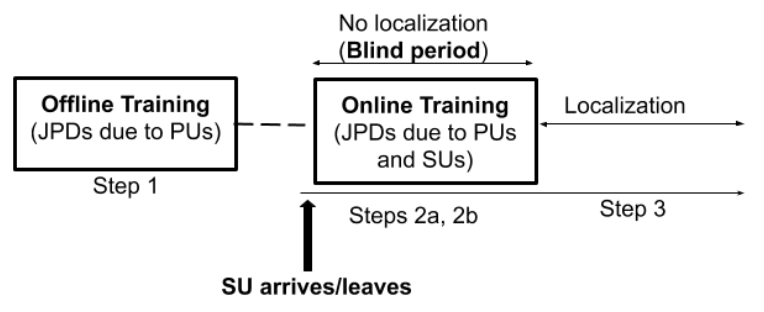
\includegraphics[width=0.7\textwidth]{chapters/ipsn/figures/map**2.png}
	\caption{\ouralgoss's overall approach}
	\label{fig:auth}
\end{figure}

\softpara{\ouralgoss: Localizing with Authorized Users}. Our problem
is to localize intruders in a shared spectrum system with fixed
primaries and changing set of secondaries.  Our \ouralgoss approach
uses a combination of a priori (offline) and online training to
construct JPDs for appropriate hypotheses based on gathered
observations, and then use these JPDs to localize intruders in
real-time using the \ouralgo approach described in the previous
section. We start with defining a few useful notations.

We use \Pa to denote the set of (fixed) primaries, and \Ka to denote
the set of secondaries at a given instant, and \ii to denote the \jth
configuration of intruders (we can assume the zero-th configuration to
represent no intruders). We use $\tau = \Pa \cup \Ka \cup \ii$ to denote the
set to all transmitters (authorized and unauthorized) at a given
instant.  Finally, we use $\pd(\vx | (\tau = X))$ to denote the joint
probability distribution (JPD) of observation vectors from the
deployed sensors when the prevailing hypothesis is that the set $\tau$
of transmitters is $X$. \ouralgoss is the sequence of following steps.
\begin{packedenumerate}
	\item
	(Offline Step.) Construct JPDs $\pd(\vx | \Pa)$ and $\pd(\vx | \tau = (\ii \cup \Pa))$ for all $j$. Since these JPDs 
	are independent of the secondaries, they do not change and
	can be done once a priori.
	\item
	(Online Steps.) Whenever \Ka (set of secondaries) changes:
	\begin{packedalpha}
		\item Construct JPD $\pd(\vx | \tau = (\Pa \cup \Ka))$. 
		\item Compute $\pd(\vx | \tau = (\Pa \cup \ii \cup
                  \Ka))$ for all $j$, from above constructed JPDs,
                  viz., $\pd(\vx | \Pa)$, $\pd(\vx | \tau = (\ii \cup
                  \Pa))$, and $\pd(\vx | \tau = (\Pa \cup \Ka))$. See
                  the below observation.
	\end{packedalpha}
	\item
	(Real-time Localization.) Periodically, each sensor sends its
          observation to a centralized entity (spectrum
          manager) which uses \ouralgo to localize any intruders
          present. Here, localization essentially means determining
          the most likely prevailing hypothesis among the hypotheses
          $\tau = (\Pa \cup \ii \cup \Ka)$, based on the JPDs $\pd(\vx | \tau = (\Pa \cup \ii \cup \Ka))$ constructed in earlier
          steps.
\end{packedenumerate}

Note that steps 1 and 2a are essentially learning the authorized users' signal charecteristics and view them as the "background signals". 
If there are no authorized users, then the background signals are "quite". Else, then the background signals have some "sound".
We now state the observation that forms the basis of JPD computation
in Steps 2b; note that the noise due to sensor's hardware gets
duplicated when ``adding'' two JPDs, but can be easily removed.
\begin{obs}
  The JPD $\pd(\vx | (\tau = A \cup B))$ and be computed from JPDs $\pd(\vx | (\tau = A))$ and $\pd(\vx | (\tau = B))$.  Similarly,
  JPD $\pd(\vx | (\tau = A))$ can be computed from the JPDs $\pd(\vx | (\tau = A
\cup B))$ and $\pd(\vx | (\tau = B))$.
\end{obs}

\para{Blind Period due to Step 2.}  Note that the steps 2a and 2b
construct or compute the JPDs needed for localization, and thus,
during their execution, the localization cannot be done. Thus, it is
important that the duration of this ``blind period'' in
minimal. Fortunately, step 2b being a simple mathematic computation
takes only in the order of milliseconds under efficient implementation, while 2a merely entails gathering a
sufficient number of observations to construct the desired JPD which
could take anywhere from milliseconds to a few seconds, as an
observation takes only a fraction of a millisecond~\cite{our-infocom}.

\para{Mobility of Users and Sensors.}  We note that \ouralgo works
seamlessly for mobile intruders and sensors, due to the constructed
PDs. However, \ouralgoss has the following limitation: the sensors
must remain static in between two consecutive online-training periods
(i.e., step 2 of above). If a sensor $X$ moves, then either $X$'s
observation must be ignored, or that $X$ needs to online-train itself
in its new location (and there should be no intruders during this
individual online-training phase). Note that active SUs are expected
to remain static anyway, as they are allocated spectrum for a specific
location.

%% . Mobility: PUs are static. (else the offline and online training needs to be redone).
%%             Active SUs static (otherwise online learning needs to be redone, if they move).
%%             Intruders can move --- each time window localizes intruders at that instant of time.
%%             Sensors. Cannot move during the period between change of active SUs. If they do, then retraining
%%                      needs to be done. 

\section{Large-Scale Simulation Results}
\label{sec:eval}

To evaluate our techniques in a large scale area (a few kms square),
we conducted simulations over a geographic area using path-loss values
from the Longley-Rice propagation model generated by
open sourse software SPLAT!~\cite{splat}. We describe the simulation setting below and
discuss the results.

\subsection{Settings}

\para{Generating Probability Distributions.} To evaluate our
techniques over a large area with 100s of sensor nodes, we need to run
simulations with an assumed propagation model. We use the well-known
Longley-Rice ~\cite{lr} Irregular Terrain With Obstruction Model (ITWOM), 
which is a complex model of wireless
propagation based on many parameters including locations, terrain
data, obstructions and soil condition etc. and such.
%%%%%%%%%%%%
We consider an area of 4km $\times$ 4km in the NY state and use the
800 MHz band for SPLAT! We discretize the area using 40 vertical and
40 horizontal grid lines---yielding 1600 cells each of size 100m
$\times$ 100m.
%\red{Each cell represents a discrete location.}
%%%%%%
To generate a probability distribution (PD) at a sensor location $x$
due to a transmitter at location $l$ transmitting at power $\pstar$,
we compute the received power at $x$ using transmit power minus path-loss from SPLAT!, and use it as the mean of the probability distribution. For the
complete PD, we assume Gaussian distributions and use a standard
deviation between 1 and 3, with higher values for pairs $(x,l)$ with
smaller distance.
%%%%%%
As mentioned before, the PD due to multiple simultaneous transmitters
can be computed as just a ``sum'' of the Gaussian distributions due to
individual transmitters~\cite{rappaport-2001,mobicom17-splot}.
%% \ble{The expectation of power of the sum of multiple signals is equal
%%  to the sum of power of the individual signals
%%  ~\cite{rappaport-2001}.  ~\cite{mobicom17-splot} validates this by
%%  conducting experiments in the Orbit testbed.}

\para{Algorithms Compared.}  For the \mtl problem, we compare our
\ouralgo algorithm with \splot~\cite{mobicom17-splot} and
\cl~\cite{clustering} (see \S\ref{sec:ipsn-related}). As mentioned
before,~\cite{Quasi-EM} has been shown to be inferior in performance
to both \splot and \cl in their respective works, and thus, not
evaluated here.
%%%%%%
\cl uses $k$-means~\cite{scikit-learn} for clustering, and needs to be
provided with the number of clusters. To do a somewhat fair
comparison, we provide \cl with a {\em range} of the number of
intruders and use the elbow-point method to pick the best
number of clusters/intruders. In particular, the range of intruders
passed to \cl is 1 to $2x$, where $x$ is the actual number of
intruders present.
%%%%%%%%%
\begin{table}[ht]
	\caption{Simulation Evaluation Parameters.}
	\centering
	\begin{tabular}{c c c c}
		\hline\hline
		Param. & Value & Description \\ [0.5ex]
		\hline
		$Q^{'}_{1}$ &  0.6   & Threshold for Procedure 1's hypothesis posterior\\ 
		$Q^{'}_{2}$ &  0.1   & Threshold for Procedure 2's hypothesis posterior\\
		$R$  & 1000 & Transmission radius when power is \pstar, (m) \\
		\pstar & 30  & Transmit power during training, (dBm) \\
		$\delta_p$ & 2  & Range of intruders' power is $[\pstar - \delta_p, \ \pstar + \delta_p]$\\
		\hline
	\end{tabular}
	\label{table:paramaters}
\end{table}

For \splot, we use the same set of parameters values as
in~\cite{mobicom17-splot} except that we use the confined area radius
to be 800m for our large area setting (\cite{mobicom17-splot} only
considered small 15m $\times$ 15m areas; 800m is roughly the maximum
transmission radius in our large-scale setting and other values
yielded worse results).
%%%%%%
Table \ref{table:paramaters} gives the main parameters of \ouralgo
used in our evaluations. Recall that the transmission radius is the
distance between the TX and RX for which the RX's RSS is at the noise
floor (we use -80dBm). \eat{Issues: Threshold for SPLOT, further explain $STD_1$ and
  $STD_2$}

\begin{figure}[ht]
	\centering
	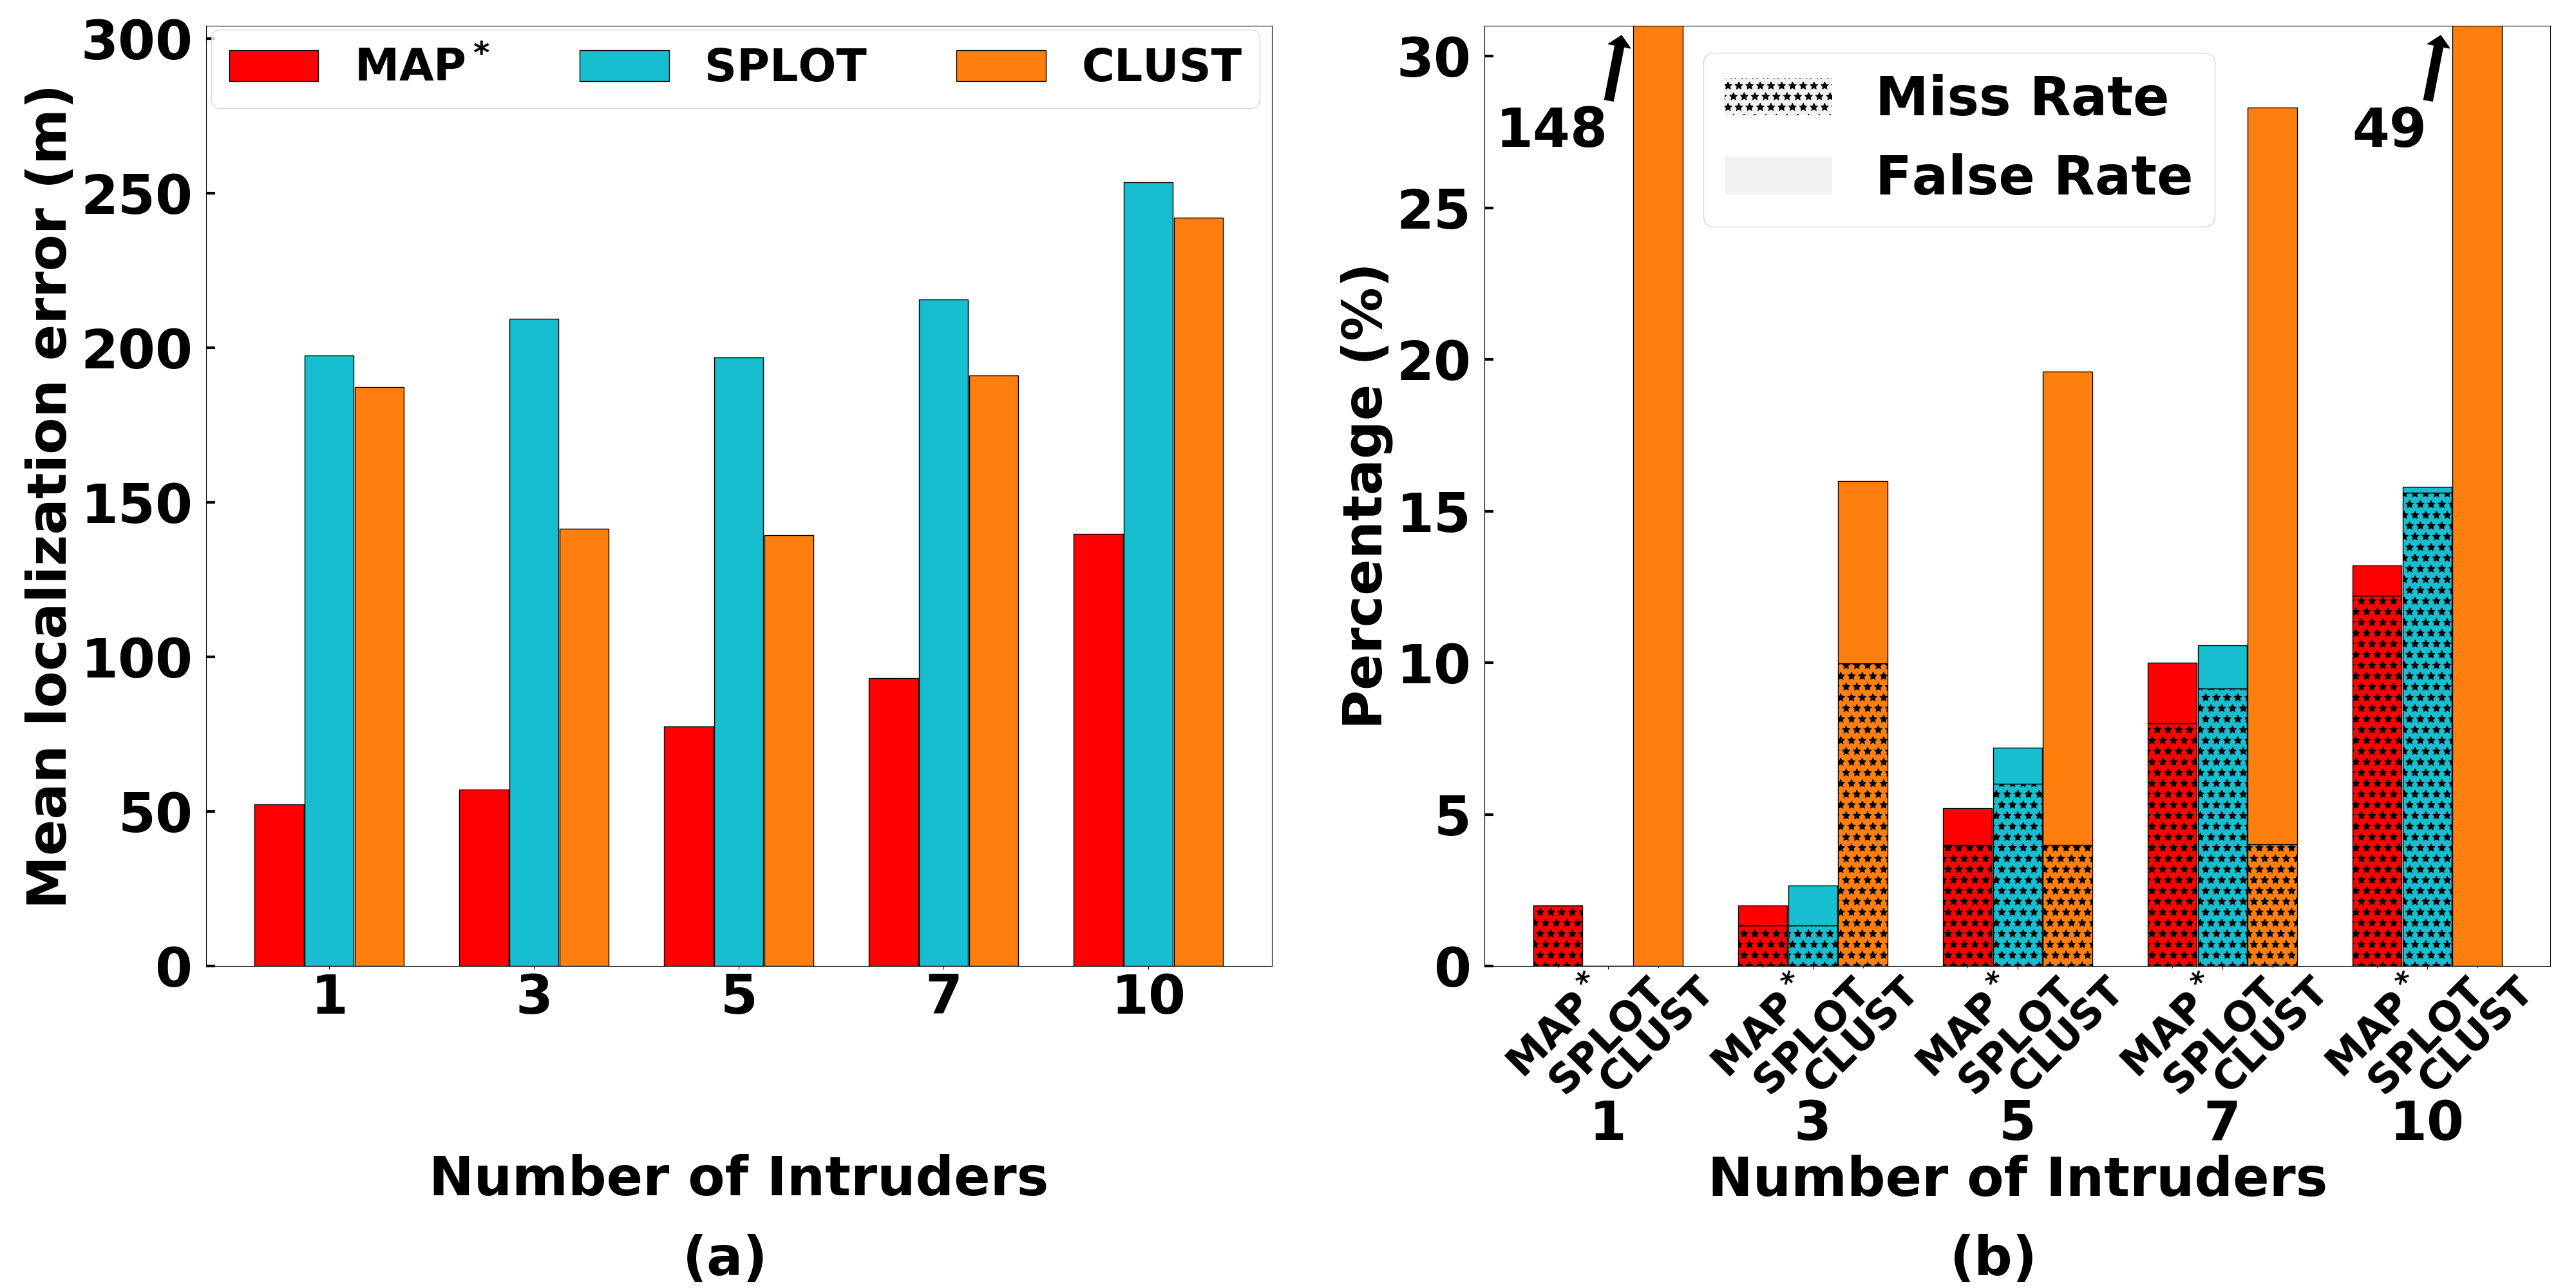
\includegraphics[width=0.8\textwidth]{chapters/ipsn/figures/splat-vary-numintru.png}
	\caption{Localization performance of various algorithms in a large scale area, for varying number of intruders}
	\label{fig:varying-num-intruders}
\end{figure}

\subsection{Five Evaluation Metrics.}
We use the following metrics to evaluate the localization methods. 
\begin{enumerate}
\item Localization error ($\lerr$). 
\item Miss rate ($\mr$).
\item False alarm rate ($\fr$).
\item Power error ($\perr$).
\end{enumerate}
The above metrics are best explained using a simple example. Given a
multi-intruder localization solution, we first compute the $\lerr$ as
the minimum-cost matching in the bi-partite graph over the
ground-truth and the solution's locations, where the cost of each edge
in the graph is the Euclidean distance. We use a simple greedy
algorithm to compute the min-cost matching.
%%%%
The unmatched nodes are regarded as false alarms or misses. E.g., if
there are 4 intruders in reality, but the algorithm predits 6
intruders then it is said to incur 0 misses and 2 false alarms and if
it predicts 3 intruders then it incurs 1 miss and 0 false alarms. The
$\mr$ and $\fr$ metrics are on a per-intruder basis, so in the above
two examples: $\mr$ is 0 and 1/4 and $\fr$ is 2/4 and 0. In the plots, we stack miss rate and false alarm rate together to show the overall difference between the true number of intruders and predicted number of intruders.
%%%%%%%
$\perr$ is the average difference between the predicted power
and the actual power of the matched pair in the above bi-partite
graph. 

Finally for interpolation schemes, we use the metric (5) interpolation error ($\ierr$) defined as the estimated path-loss minus the ground-truth path-loss value.

\subsection{Results}

In this subsection, we evaluate the performance of our techniques for
varying parameter values, viz., number of intruders and sensors in the
field, and training cost.
%%%%%%%%
Here, the training cost is defined relative (specifically, as a
percentage of) to the full training scenario wherein we construct each
of the $1600 \times 1600$ PDs (one for each pair of transmitter and
sensor locations) directly from observations. E.g., $x\%$ training
cost indicates that we construct $1600 \times (16x)$ PDs directly, and
interpolate the remaining $1600 \times (1600-16x)$ PDs; our proposed
interpolation scheme only interpolates for sensor locations.
%%%%%%
In general, when we vary a specific parameter, the other parameters
are set to their default values which are: 9\% for training
cost, 5 for number of intruders, and 240 for number of sensors.
%%%%%
For each experiment, the said number of sensors and intruders are
deployed randomly in the field, with the intruders deployed in the
continuous location domain while the sensors deployed only at the
centers of the grid cells. Each data point in the plots is an
average of 50 experiments.

\begin{figure}[ht]
	\centering
	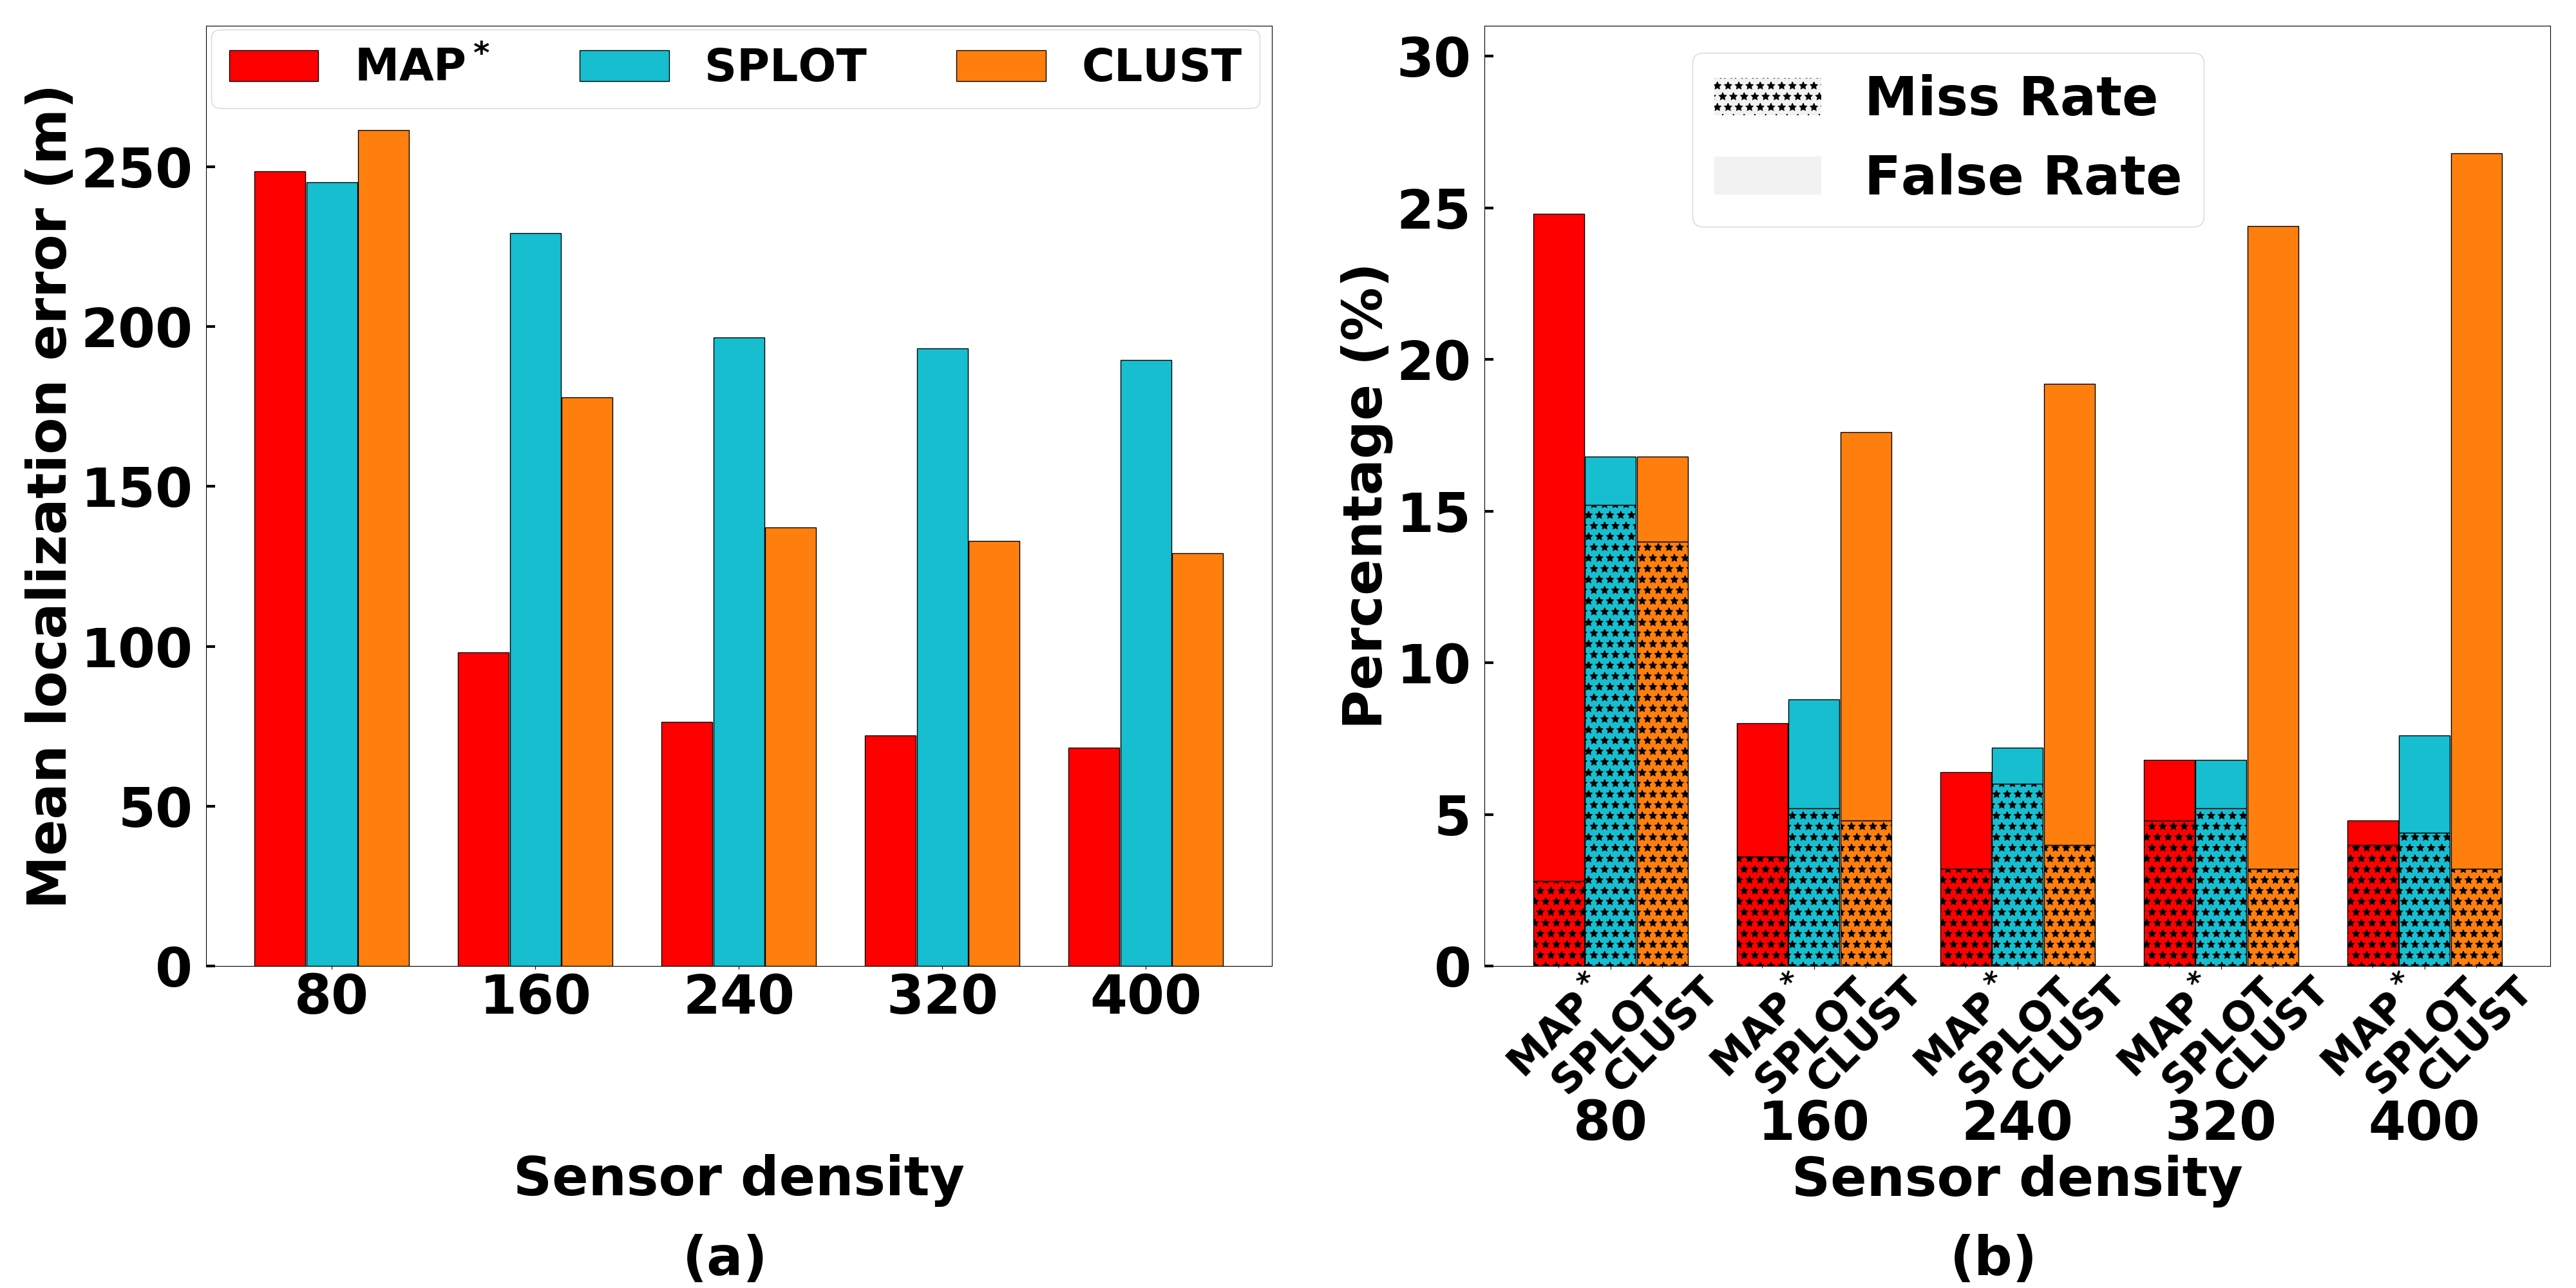
\includegraphics[width=0.8\textwidth]{chapters/ipsn/figures/splat-vary-sendensity.png}
	\caption{Localization performance of various algorithms in a large scale area, for varying sensor density}
	\label{fig:varying-num-sendensity}
\end{figure}

\para{Varying Number of Intruders.}  First, we compare the
localization accuracy of various algorithms for varying number of
intruders.  See Figure \ref{fig:varying-num-intruders}. We vary the
number of intruders from 1 to 10. We observe that the localization
error of \ouralgo is the minimum across the three algorithm. 
The localization error is 45\% -- 74\% less than \splot.
In terms of the $\mr$ and $\fr$, \ouralgo also performs others which confirms the overall performance
of \ouralgo to be the best among the algorithms compared. In terms of
absolute performance, note that the localization error of 50-150m
indicates an error of 1-2 grid cells, and thus is minimal in the
context of the large area of 4km by 4km with 1600 cells and a sensor
population of 240. Investigating further, we observe that misses in
\ouralgo are mostly due to the interpolated PDs (note that only 9\% of
the PDs are constructed from the actual sensor observations, and the
remaining 91\% are interpolated), while \splot's misses are mainly
from the case of two or more intruders being close to each other. This
demonstrates the superior ability of \ouralgo to localize intruders
that are close-by via the designed sequence of Procedures 1 and 2.


\begin{table}
	\caption{\ouralgo Power Error (dB) }
	\centering
	\begin{tabular}{c c c} 
		\hline\hline
		\# Intru. & MAE & ME \\ [0.5ex]
		\hline
		1 & 0.56  & -0.07  \\ 
		3 & 1.02  & 0.89 \\
		5 & 1.31  & 0.97 \\
		7 & 1.52  & 1.16 \\
		10 & 1.47 & 1.04 \\
		\hline
	\end{tabular}
	\label{table:splat-power-error}
\end{table}

\begin{table}
	\caption{Running time (s)}
	\centering
	\begin{tabular}{c c c c}
		\hline\hline
		\# Intru. & \ouralgo & \splot & \cl \\
		\hline
		1 &  0.55 & 0.56 & 0.03\\ 
		3 &  1.07 & 1.02 & 0.11  \\
		5 &  5.74 & 1.35 & 0.23 \\
		7 &  8.14 & 1.63 & 0.30 \\
		10 & 16.50 & 1.89 & 0.41  \\
		\hline
	\end{tabular}
	\label{table:splat-running-time}	
\end{table}


\softpara{Intruder Power Estimation, and Computation Time.}
Table~\ref{table:splat-power-error} shows the mean absolute error
(MAE) and mean error (ME) of the intruder's predicted power by
\ouralgo. Note that \cl and \splot do not predict intruder's power,
and hence, not shown. We observe that \ouralgo is able to predict
intuder's power quite accurately. The errors increase with the increase in number of intruders. Also, the mean error begins at near zero and then turns positive. 
%%%%%
Table~\ref{table:splat-running-time} shows the running time of various
algorithms over an Intel i7-8700 3.2 GHz processor. We see that \cl is
the fastest, and the running times of \ouralgo and \splot are
comparable for small number of intruders, but for larger number of
intruders, \ouralgo takes longer time than \splot mainly because of
more number of iterations of the computationally-intensive Procedure
2.

\begin{figure}[ht]
	\centering
	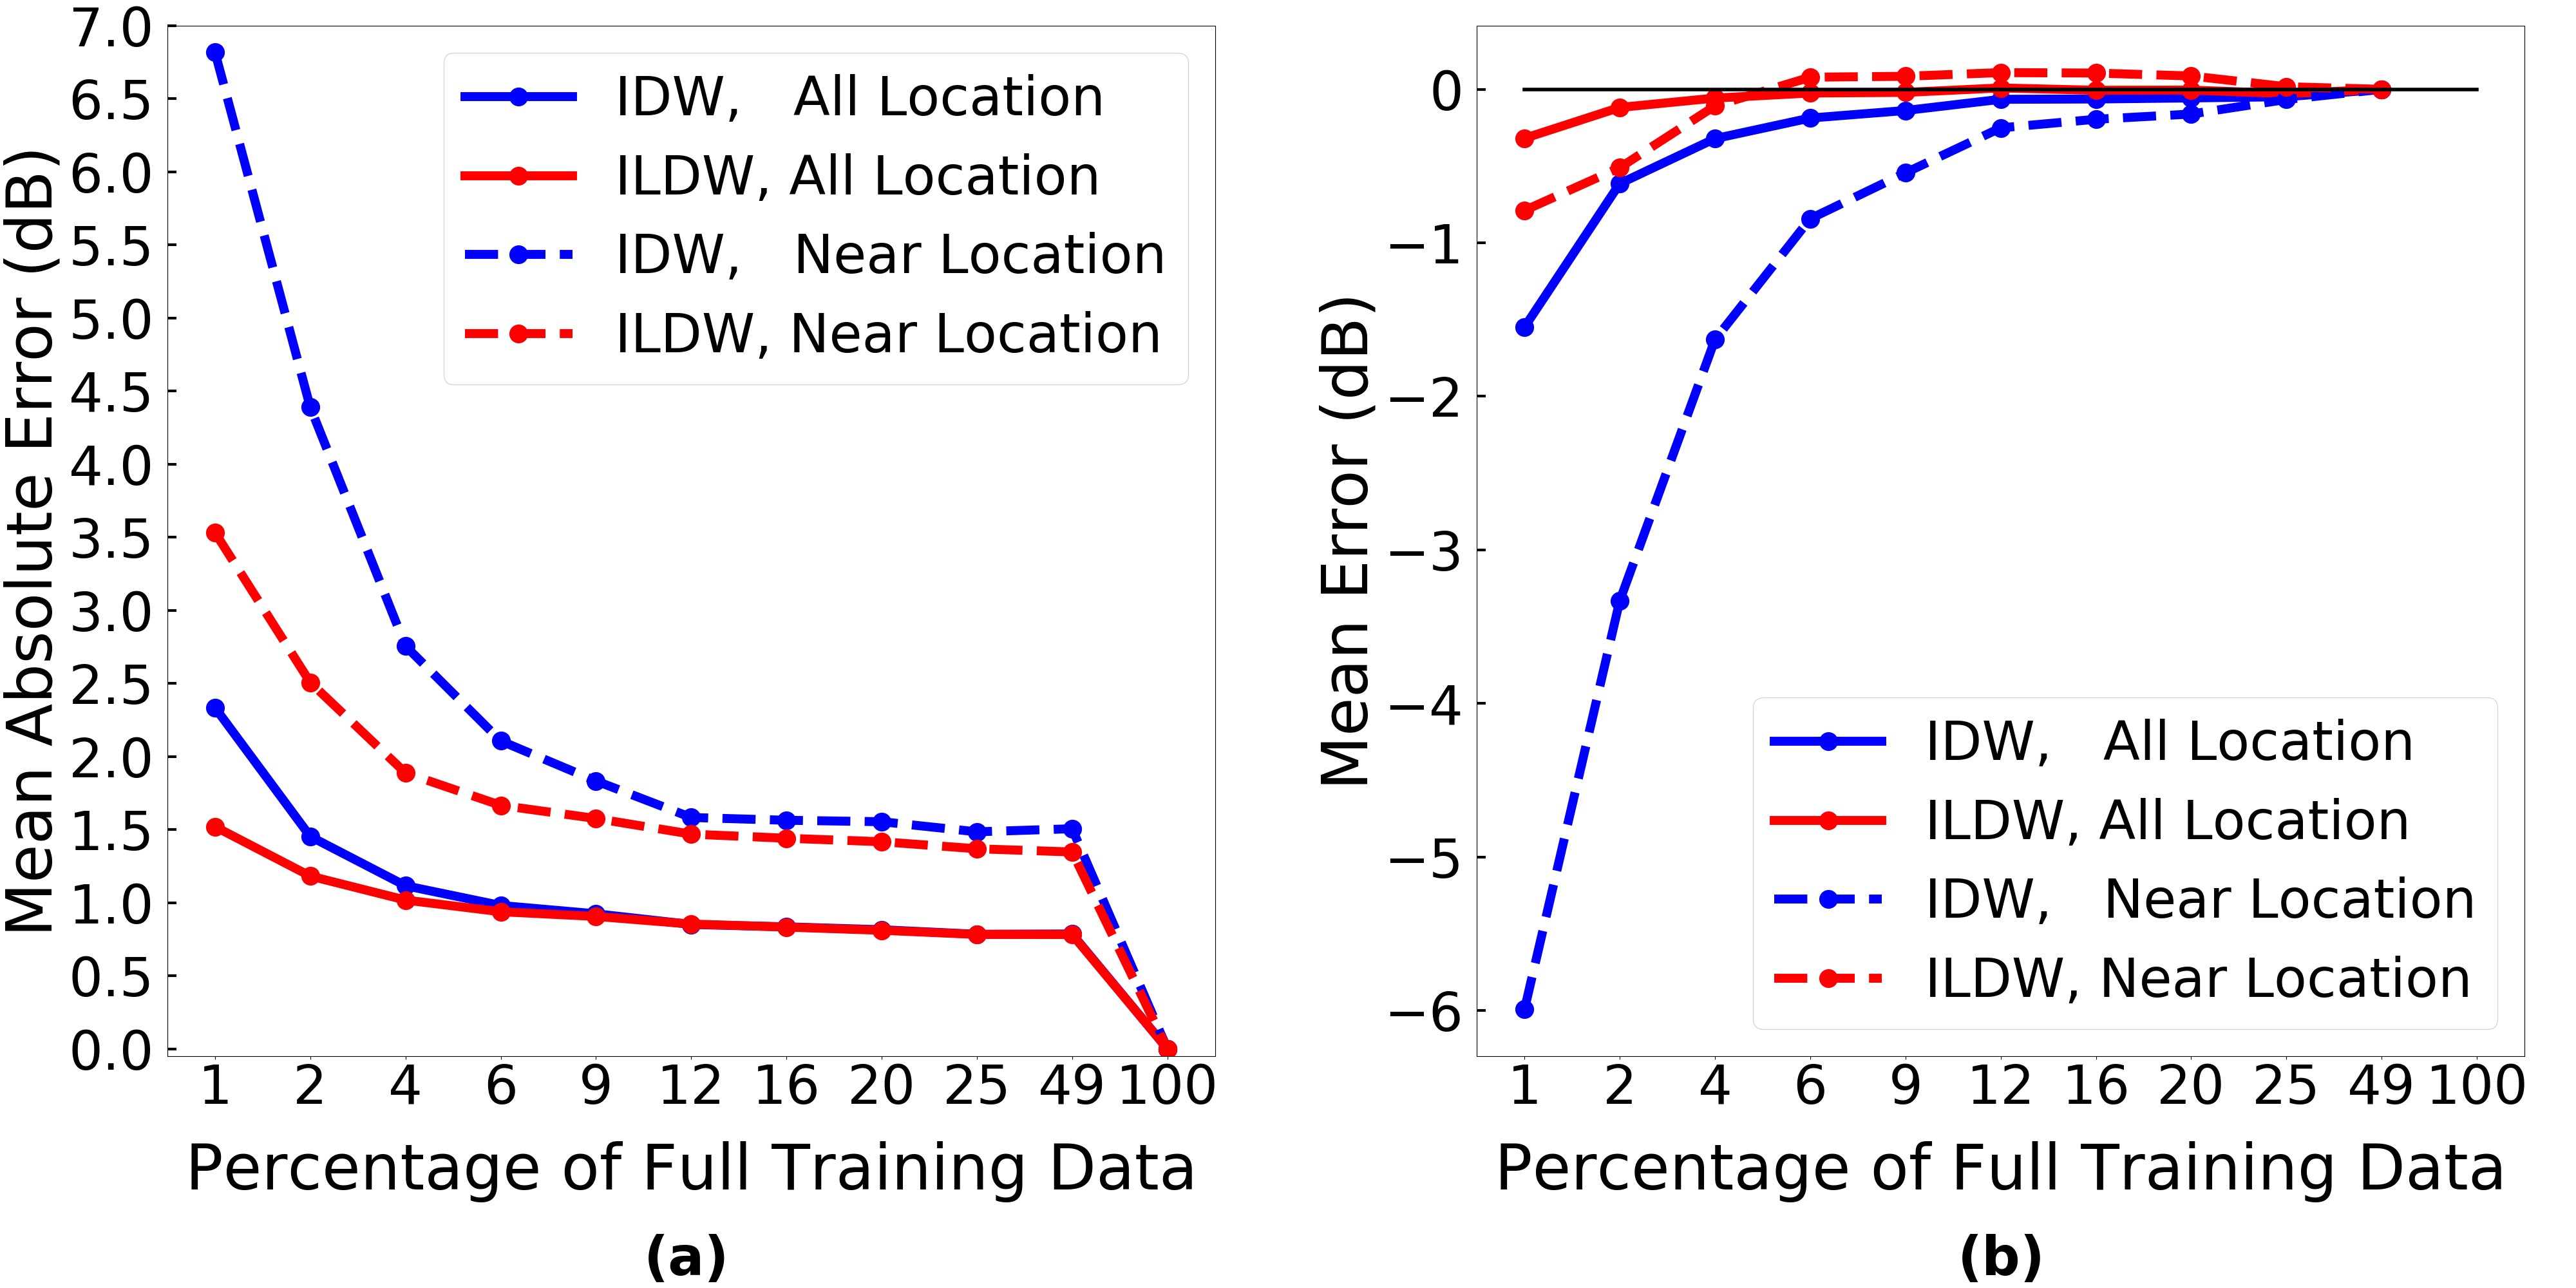
\includegraphics[width=0.8\textwidth]{chapters/ipsn/figures/inter_error.png}
	\caption{Estimation errors for interpolation schemes for varying training data}
	\label{fig:inter-error}
\end{figure}

\para{Varying Sensor Density.} We now vary the total number of sensors
in the field, and observe the impact on the performance of various
algorithms. See Figure \ref{fig:varying-num-sendensity}, where the
number of sensors is varied from 80 to 400. We see that all algorithms
perform better with increasing number of sensors as expected, with
\ouralgo performance improving significantly (in both $\lerr$ as well
as $f_r + m_r$) as number of sensors is increased from 80 to 160. More
importantly, except for very low number of sensors (i.e., 80),
\ouralgo handily outperforms the other two algorithms.


\para{Varying Training Cost.}  Finally, we now investigate how the
training cost (i.e., number of PDs constructed from raw observations)
affects the performance of our \ouralgo algorithm. Note that the other
algorithms do not depend on the training data, hence not shown.
%%%%%%%%%%
We first evaluate the interpolation error of our \ildw scheme for
varying training cost (number of known PDs) by comparing with the
traditional IDW scheme on which it is based. See
Figure~\ref{fig:inter-error}, which plots the mean absolute error
(MAE) as well as mean error (ME). As the interpolation error is
substantially higher for points that are closer to the transmitter, we
plot MAE and ME as averaged over all interpolated points as well as
over just the points close (less than 800m away) to the transmitter. Note
that the PDs at sensor locations closer to the transmitter would have
a stronger bearing on the localization accuracy, and thus, the MAE and
ME values for points closer to the transmitter are of more
significance.
%%%%%
We observe here that as expected both MAE and (absolute value of) ME
decrease with increase in the training cost for both \idw and \ildw,
but MAE and ME of \ildw is significantly lower than that of \idw
especially for low percentages of training cost and when the points
are close to the transmitter.
%\rd{HG: I want to remove the following
 % sentence.}  \ble{This shows that weighting the neighbors in the
  %logarithm scale towards the transmitter mitigates the negative
  %trend.}

We now plot the performance of \ouralgo for varying training data; see
Figure~\ref{fig:varying-training-data}. As expected, the performance
metrics show general improvement with increase in amount of
training. More importantly, we note that with 5-10\% of training,
\ouralgo achieves performance comparable to that with 100\% training,
suggesting that our interpolation scheme is largely effective as long
as 5-10\% of PDs are constructed from raw observations. 
\eat{TODO \red{Put Fig 7+8,
  9+10 in the same ROWs as Fig 7(a)-(b) and 8(a)-(b). will look better.}}



\begin{figure}[ht]
	\centering
	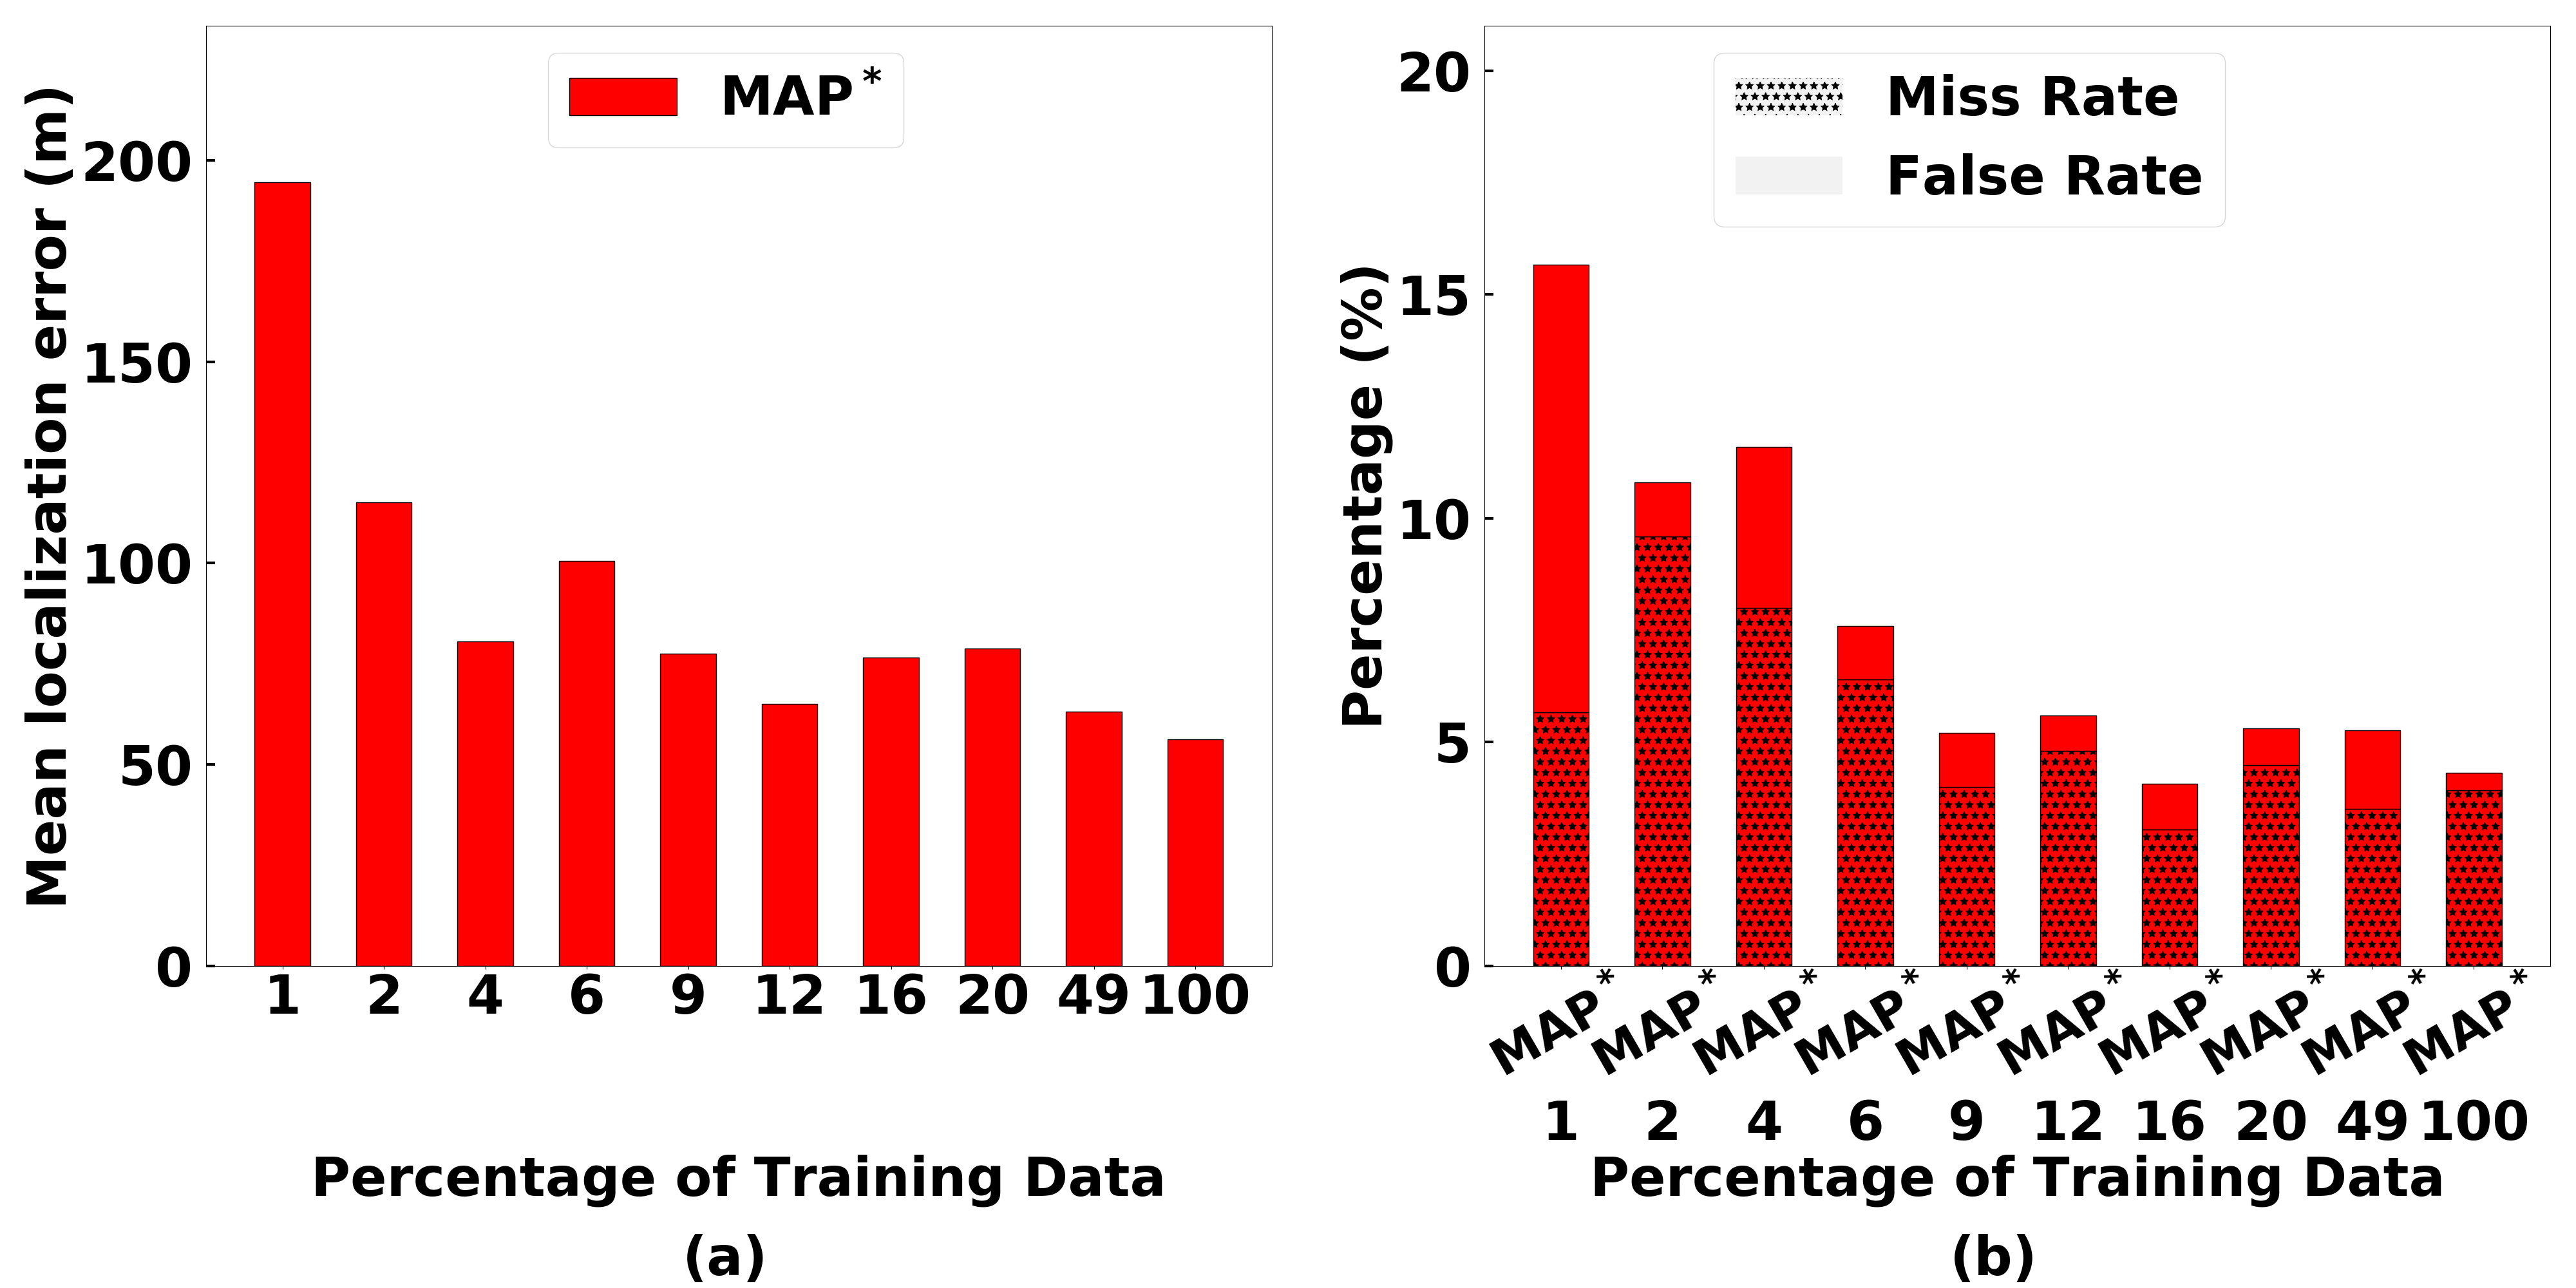
\includegraphics[width=0.8\textwidth]{chapters/ipsn/figures/splat-vary-training.png}
	\caption{Localization performance of \ouralgo in a large scale area, for varying training data}
	\label{fig:varying-training-data}
\end{figure}

\para{In Presence of Authorized Users (\ouralgoss).}  We now evaluate
the performance of our \ouralgoss approach which is tailored to work
in the presence of authorized users. To evaluate \ouralgoss, we place
5 authorized users in the area---with 2 primary and 3 secondary users.
The primary users are placed at fixed locations, while the secondaries
are put at random locations. We assign each authorized user a random
power in the range of 30 to 32dBm, while, as before, a random power
between 28 and 32dBm to the intruders. To ensure that these 5
authorized users do not ``interfere'' with each other, we ensure that
the distance between any two of these authorized users is at least
1000m.
%%%%%%%%%
We compare \ouralgoss with the simpler approach called \ouralgos that
uses \ouralgo to localize all transmitters (authorized as well as
intruders) and then removes the predicted transmitters that are
closest to the authorized users.
%%%
See Figure \ref{fig:shared-spectrum}, which shows that \ouralgoss easily
outperforms \ouralgos for varying number of intruders. 

\begin{figure}[ht]
	\centering
	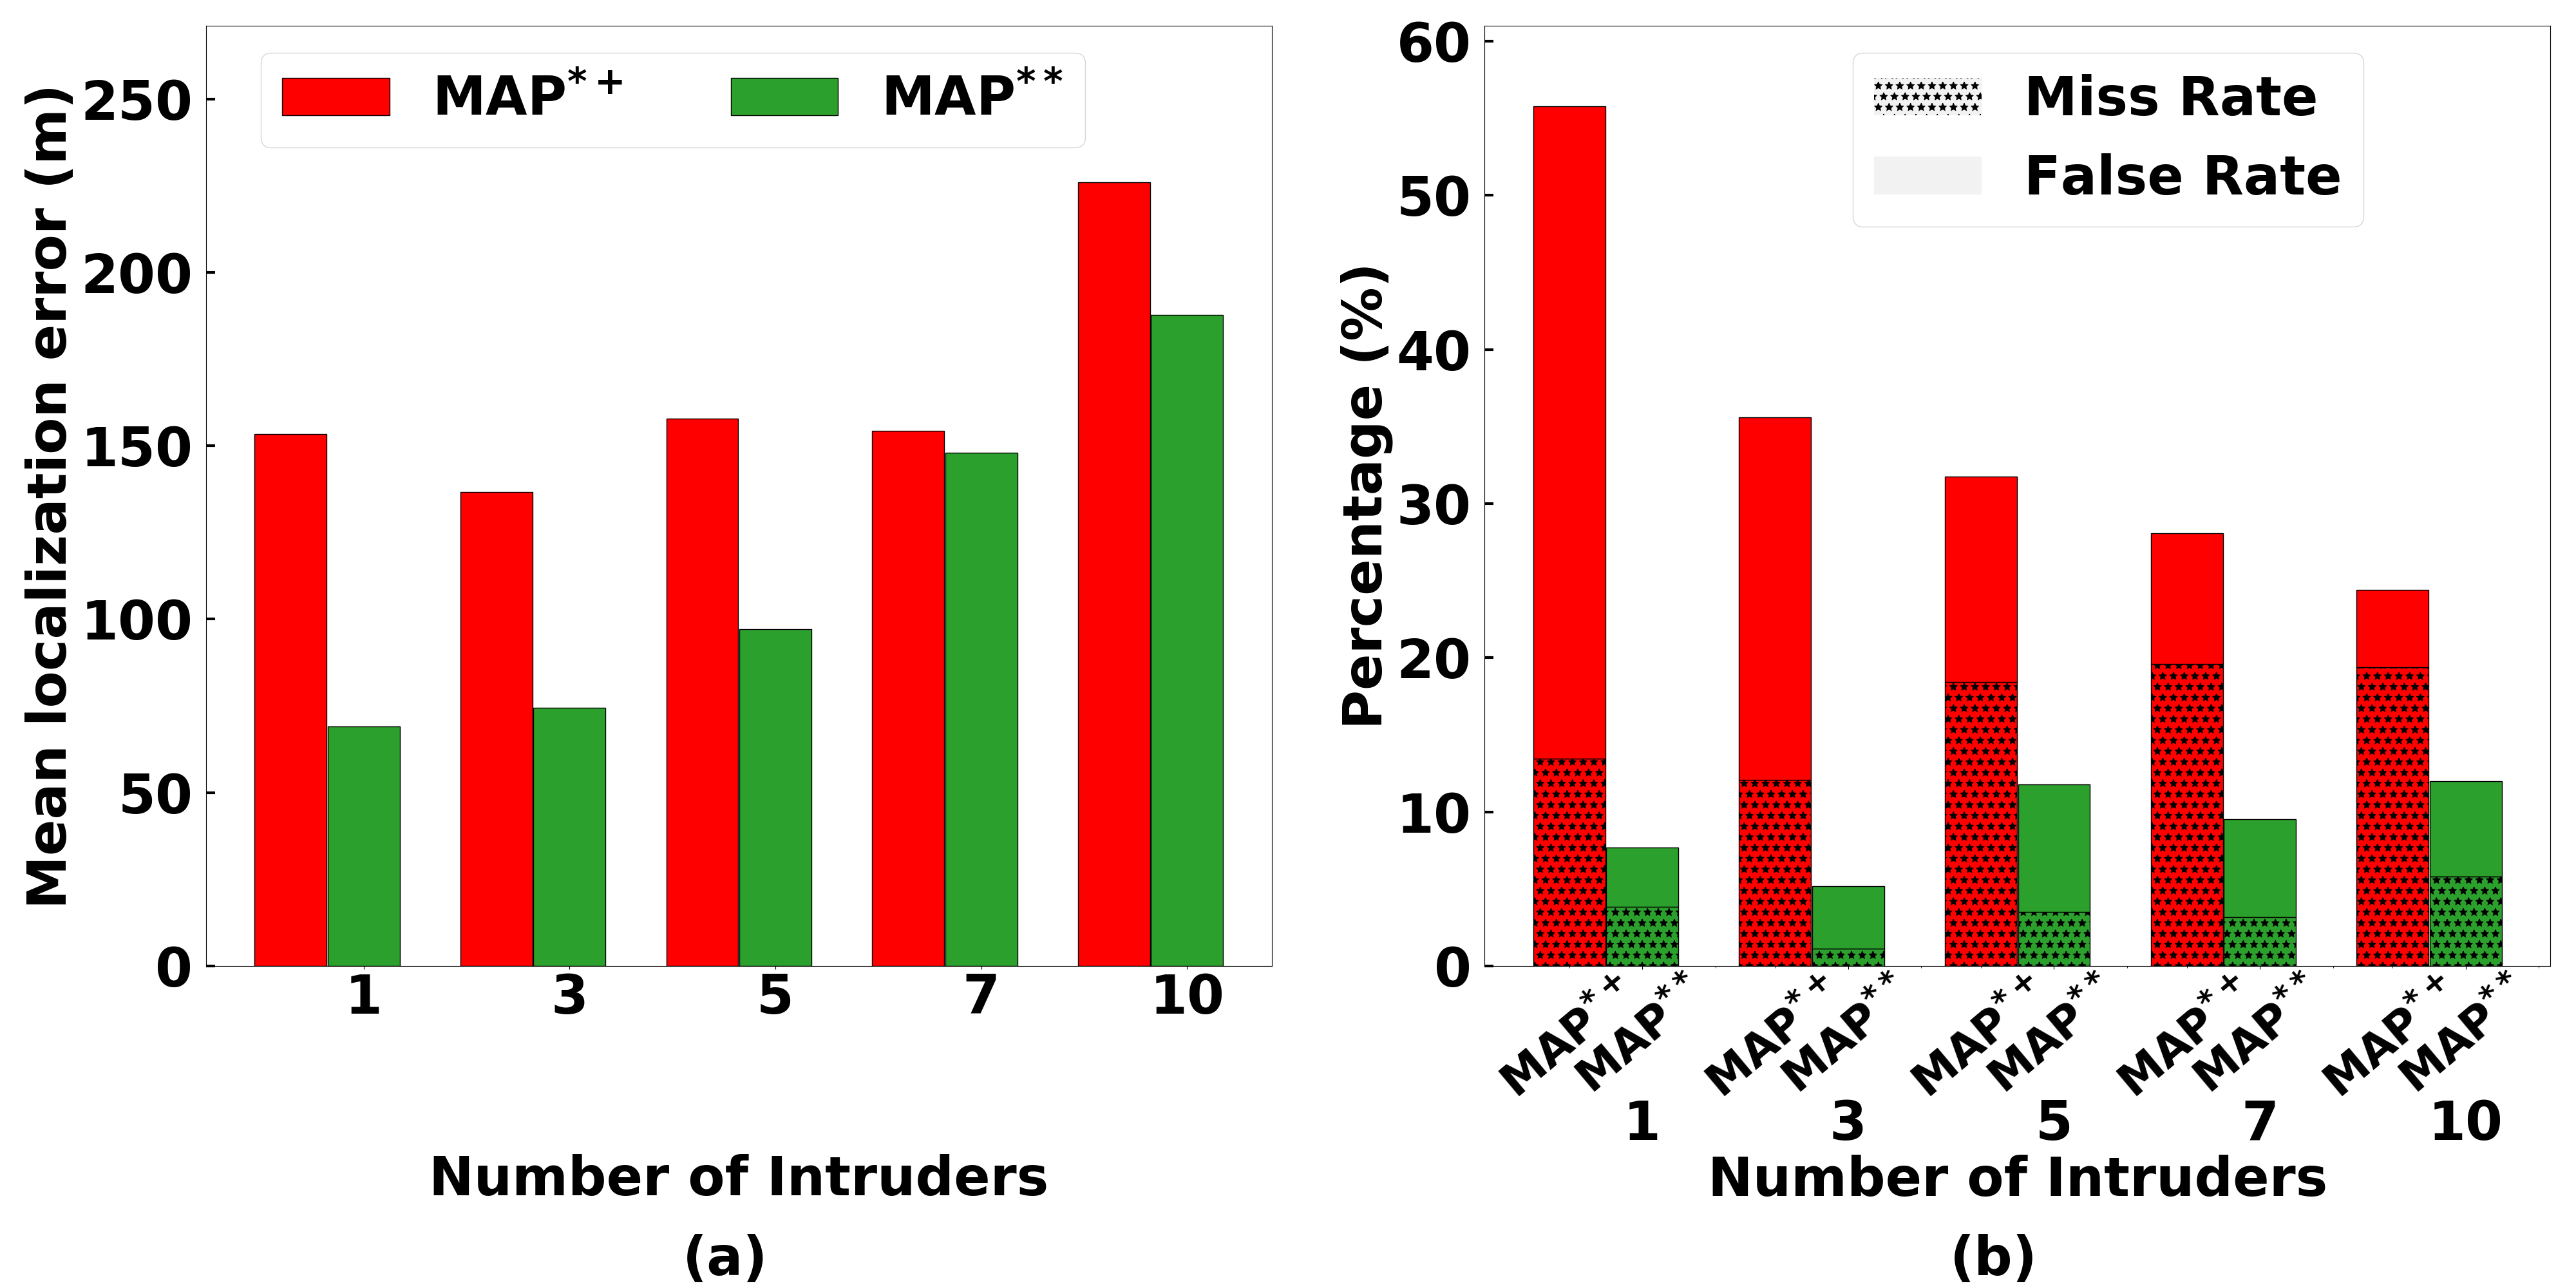
\includegraphics[width=0.8\textwidth]{chapters/ipsn/figures/splat-vary-numauthorized.png}
	\caption{Localization performance of \ouralgos and \ouralgoss in large-scale simulations with authorized users present, for varying number of intruders}
	\label{fig:shared-spectrum}
\end{figure}

\section{Testbed Implementation}
\label{sec:testbed}

In this section, we implement our techniques over commodity devices
and evaluate them over two small-scale testbeds---one indoor and one
outdoor.  Outdoor environment is a realistic setting for our target
application of shared spectrum systems, while the indoor environment
provides more challenging signal attenuation characteristics due to
walls and other obstacles.

\para{Sensor and Transmitters Used.}  Our low-cost (sub \$100, see~\cite{pam19-lowcostsensing} for a measurement study of low-cost spectrum sensors)
sensing device  is composed of a single-board computer
Odroid-C2 with an RTL-SDR dongle that
connects to a dipole antenna. We deploy 18 of these sensing devices
in our indoor and outdoor testbeds and configure them for low gain.
%The RTL-SDR devices has a noise floor of \ble{-48dB.}
%%%%%
For transmitters/intruders, we use USRP B210 and HackRF devices
  powered by laptops; we place these on a cart for mobility. These
  transmitter devices are uncalibrated, and there is no way to assign a
  specific transmit power. However, they have a configurable parameter
  called {\em gain} which is almost perfectly correlated to power when
  the gain is in a specific range, i.e., when the transmitter's gain
  is increased by 1, the receiver's signal strength increases by
  1dB. We thus use the gain parameter to adjust transmit power in the
  USRP devices. For indoor experiments, the location is manually
  derived, while for outdoor experiments, we use GPS
  dongles connected to the laptops. For collecting sensor
  observations, we implemented a Python repository in Linux that
  measures spectrum in real time at 915MHz ISM band and 2.4Msps
  sample rate.  The repository collects I/Q samples fetched from the
  RTL-SDR dongle and computes the RSS value, then records the RSS along
  with timestamp and location.  These three pieces of information are
  sent to a server that runs the localization algorithms. 

\begin{figure}
	\centering
	\begin{subfigure}[t]{0.45\textwidth}
		\includegraphics[width=\textwidth]{chapters/ipsn/figures/indoor.jpg}
		\caption{Indoor lab environment}
	\end{subfigure}
	\qquad
	\hspace{-0.15in}
	\begin{subfigure}[t]{0,42\textwidth}
		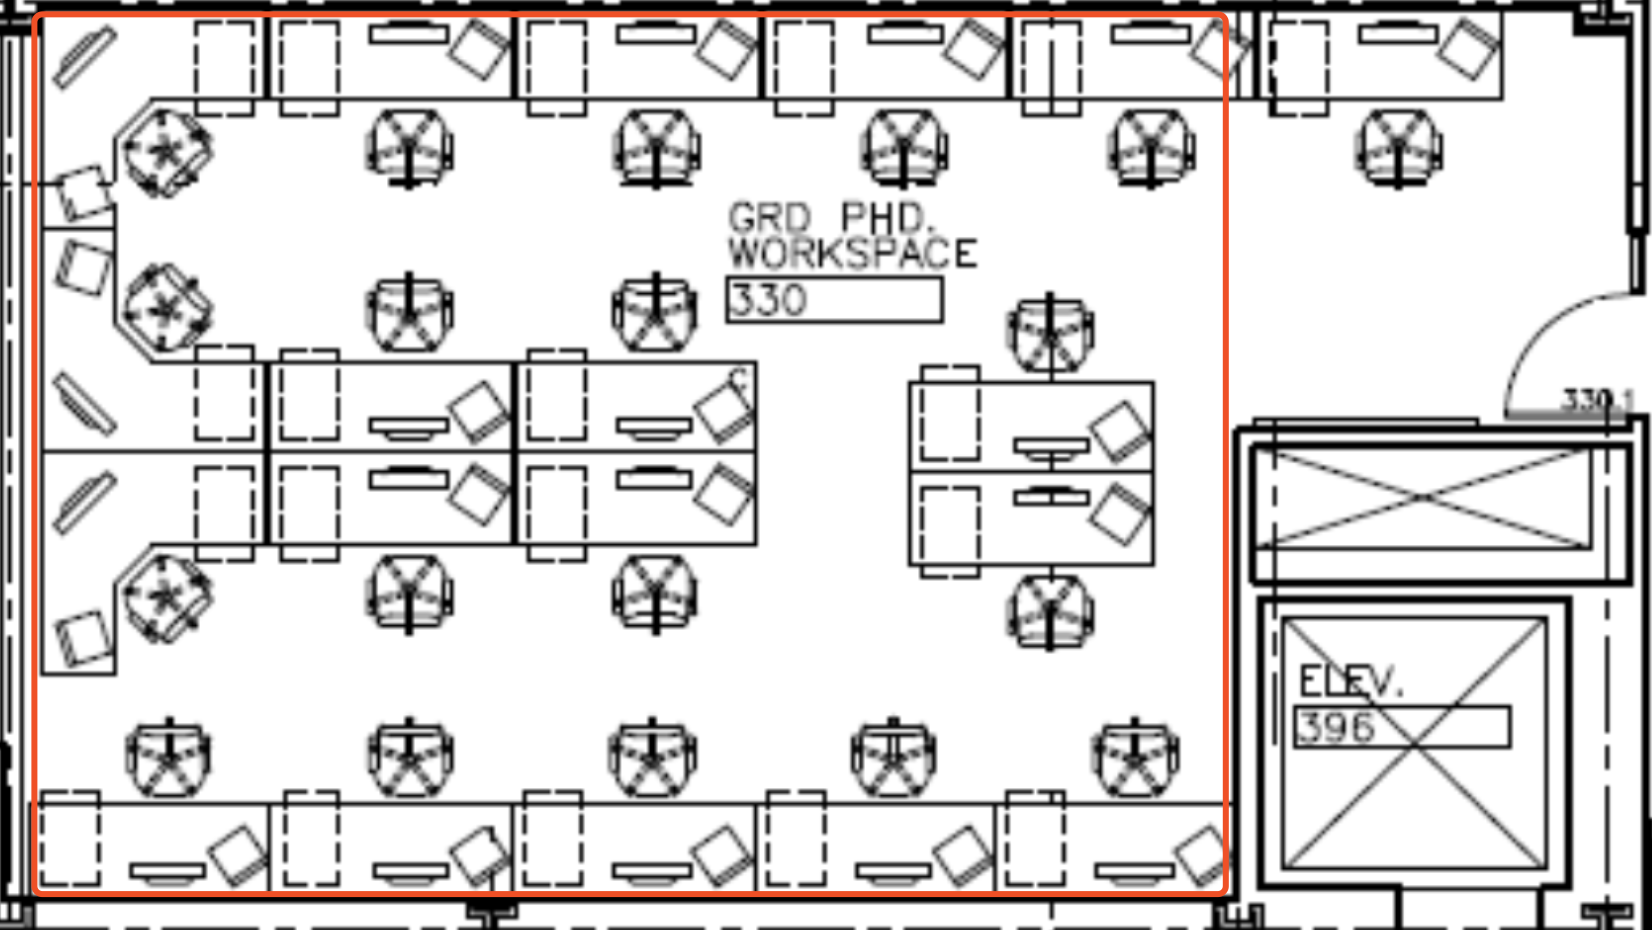
\includegraphics[width=\textwidth]{chapters/ipsn/figures/floor-plan.png}
		\caption{Floor plan}
	\end{subfigure}
	\caption{Indoor testbed. (a) Our lab used for the indoor testbed, (b) The lab's floor plan.}
	\label{fig:indoor}
\end{figure}

\begin{figure}
	\centering
	\begin{subfigure}[t]{0.585\textwidth}
		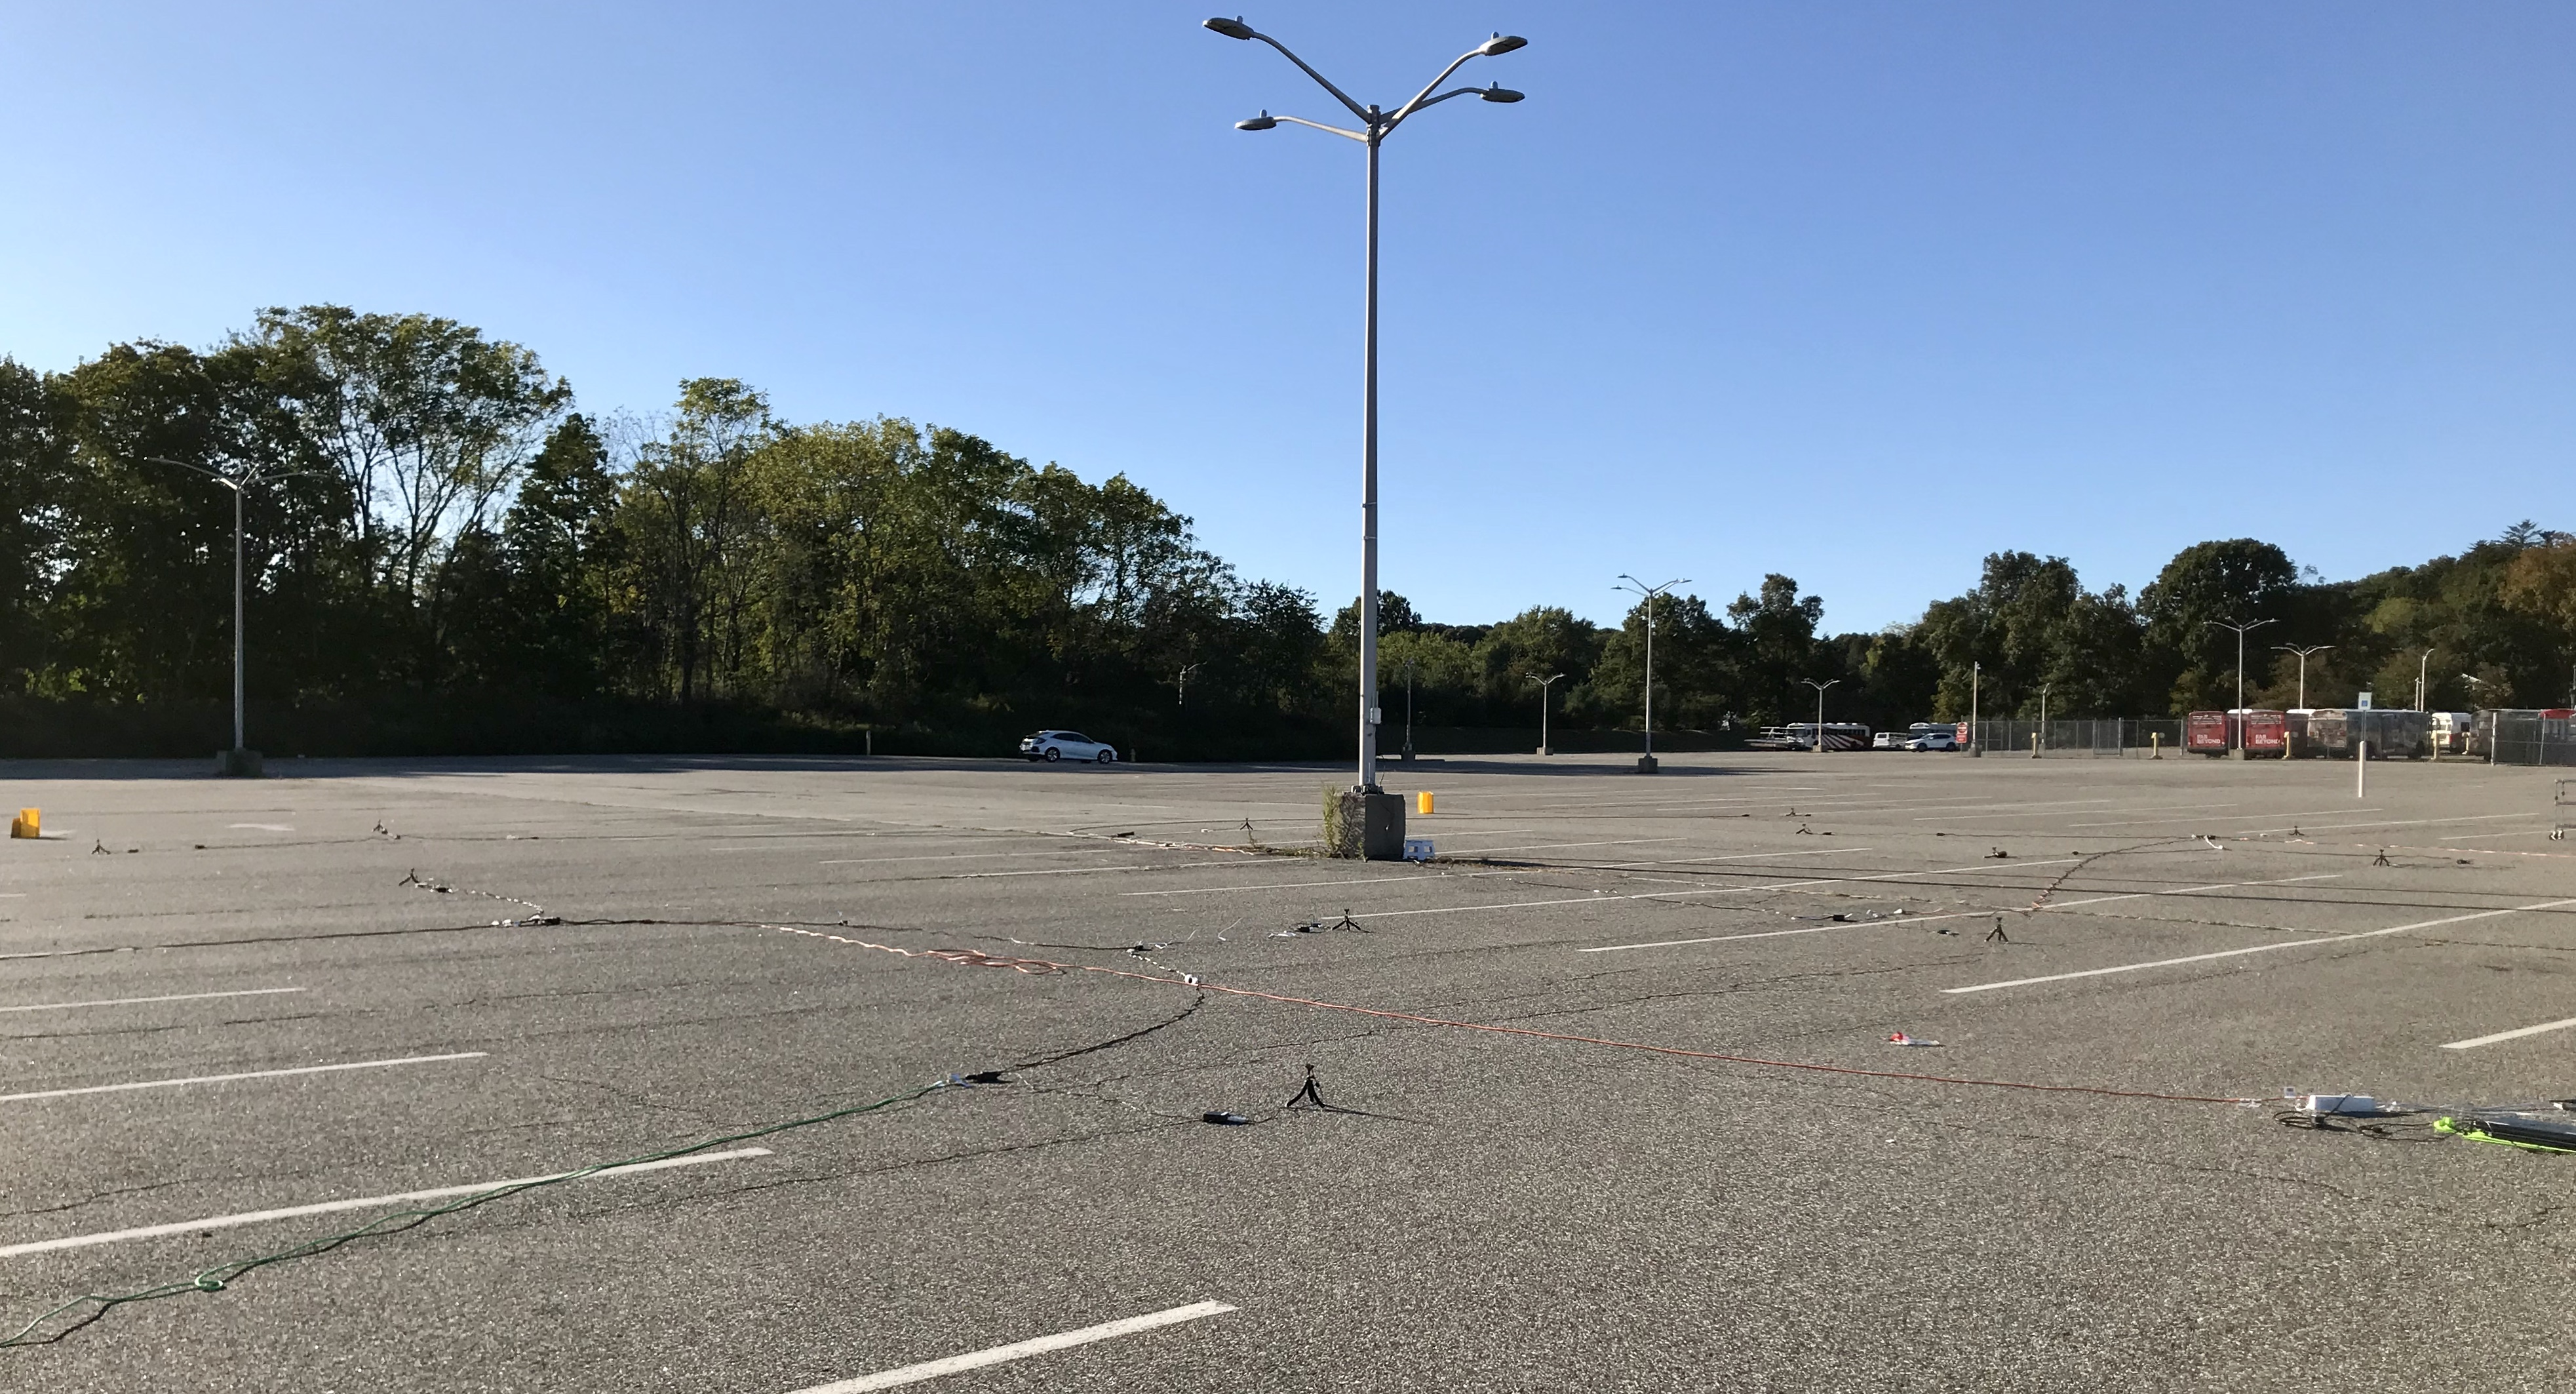
\includegraphics[width=\textwidth]{chapters/ipsn/figures/outdoor.jpg}
		\caption{Outdoor parking lot environment}
	\end{subfigure}
	\qquad
	\hspace{-0.15in}
	\begin{subfigure}[t]{0.33\textwidth}
		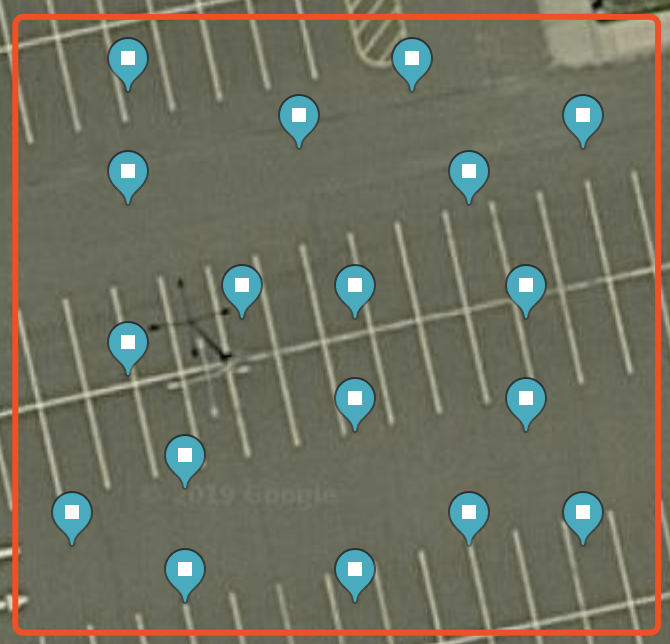
\includegraphics[width=\textwidth]{chapters/ipsn/figures/outdoor-sate.png}
		\caption{Satellite}
	\end{subfigure}
	\caption{Outdoor testbed. (a) Parking lot picture, (b)
          Satellite image of the parking lot; the red box is the area
          of the experiment, and the stars are the locations of
          sensing devices during evaluation.}
	\label{fig:outdoor}
\end{figure}

\para{Testbeds.} The {\bf indoor} testbed is built in a lab of our
Computer Science building.  Figure \ref{fig:indoor} depicts the lab
with its floor plan. The red box in the floor plan is the area where
experiments are conducted. The area is 9.6 $\times$ 7.2 $m^2$ (or 2177
square feet) large, with four rows of desks. The middle two rows
are separated by a wooden board. The area is imagined to be divided
into 48 grid cells each of size 1.2m $\times$ 1.2$m$, with the help of
ceiling tiles each of which is 0.6m $\times$ 0.6 $m$. 
%%%%
The {\bf outdoor} testbed is over an open space parking lot.  See
Figure~\ref{fig:outdoor}. The area is 32m $\times$ 32m. We divide the
area into 100 grid cells with each cell representing an area of 3.2m
$\times$ 3.2m. The GPS device returns the location in (latitude,
longitude) and the program converts it into coordinates. We use an
outdoor WiFi router and long power cords for network and electrical
connection respectively.
%%%%%%%
During the evaluation, the 18 sensing devices are placed on the ground
and are randomly spread out.


\para{Training.} In both the testbeds, for training (i.e.,
constructing non-interpolated PDs), we first pick 18 random grid cells
and place sensors in their approximate centers. Then, we manually move
the transmitter around in a cart through each of the grid cells. For
the USRP transmitter, we use a gain value of 45 in the indoor
environment and 58 in the outdoor testbed. We use a higher gain for
outdoors to allow the transmitter to have a larger transmission range
in a larger area.
%%%%%%
With each grid cell, the transmitter transmits from 3 to 4 different
points within each grid cell, and for each such location of the
transmitter, the sensors (at the 18 picked locations) gather tens of
signal strength readings. From these readings, we construct a Gaussian
probability distribution from each grid cell location of the
transmitter.
%%%%
More specifically, for a particular grid cell location of the
transmitter, we average over the readings from multiple TX positions
within that particular grid cell---this process of averaging different
positions of the TX inside a grid cell makes the Gaussian
distributions more robust to multipath fading and shadowing. The
overall training process takes an hour for indoors, and about two and
a half hours for outdoors.

\begin{figure}[ht]
	\centering
	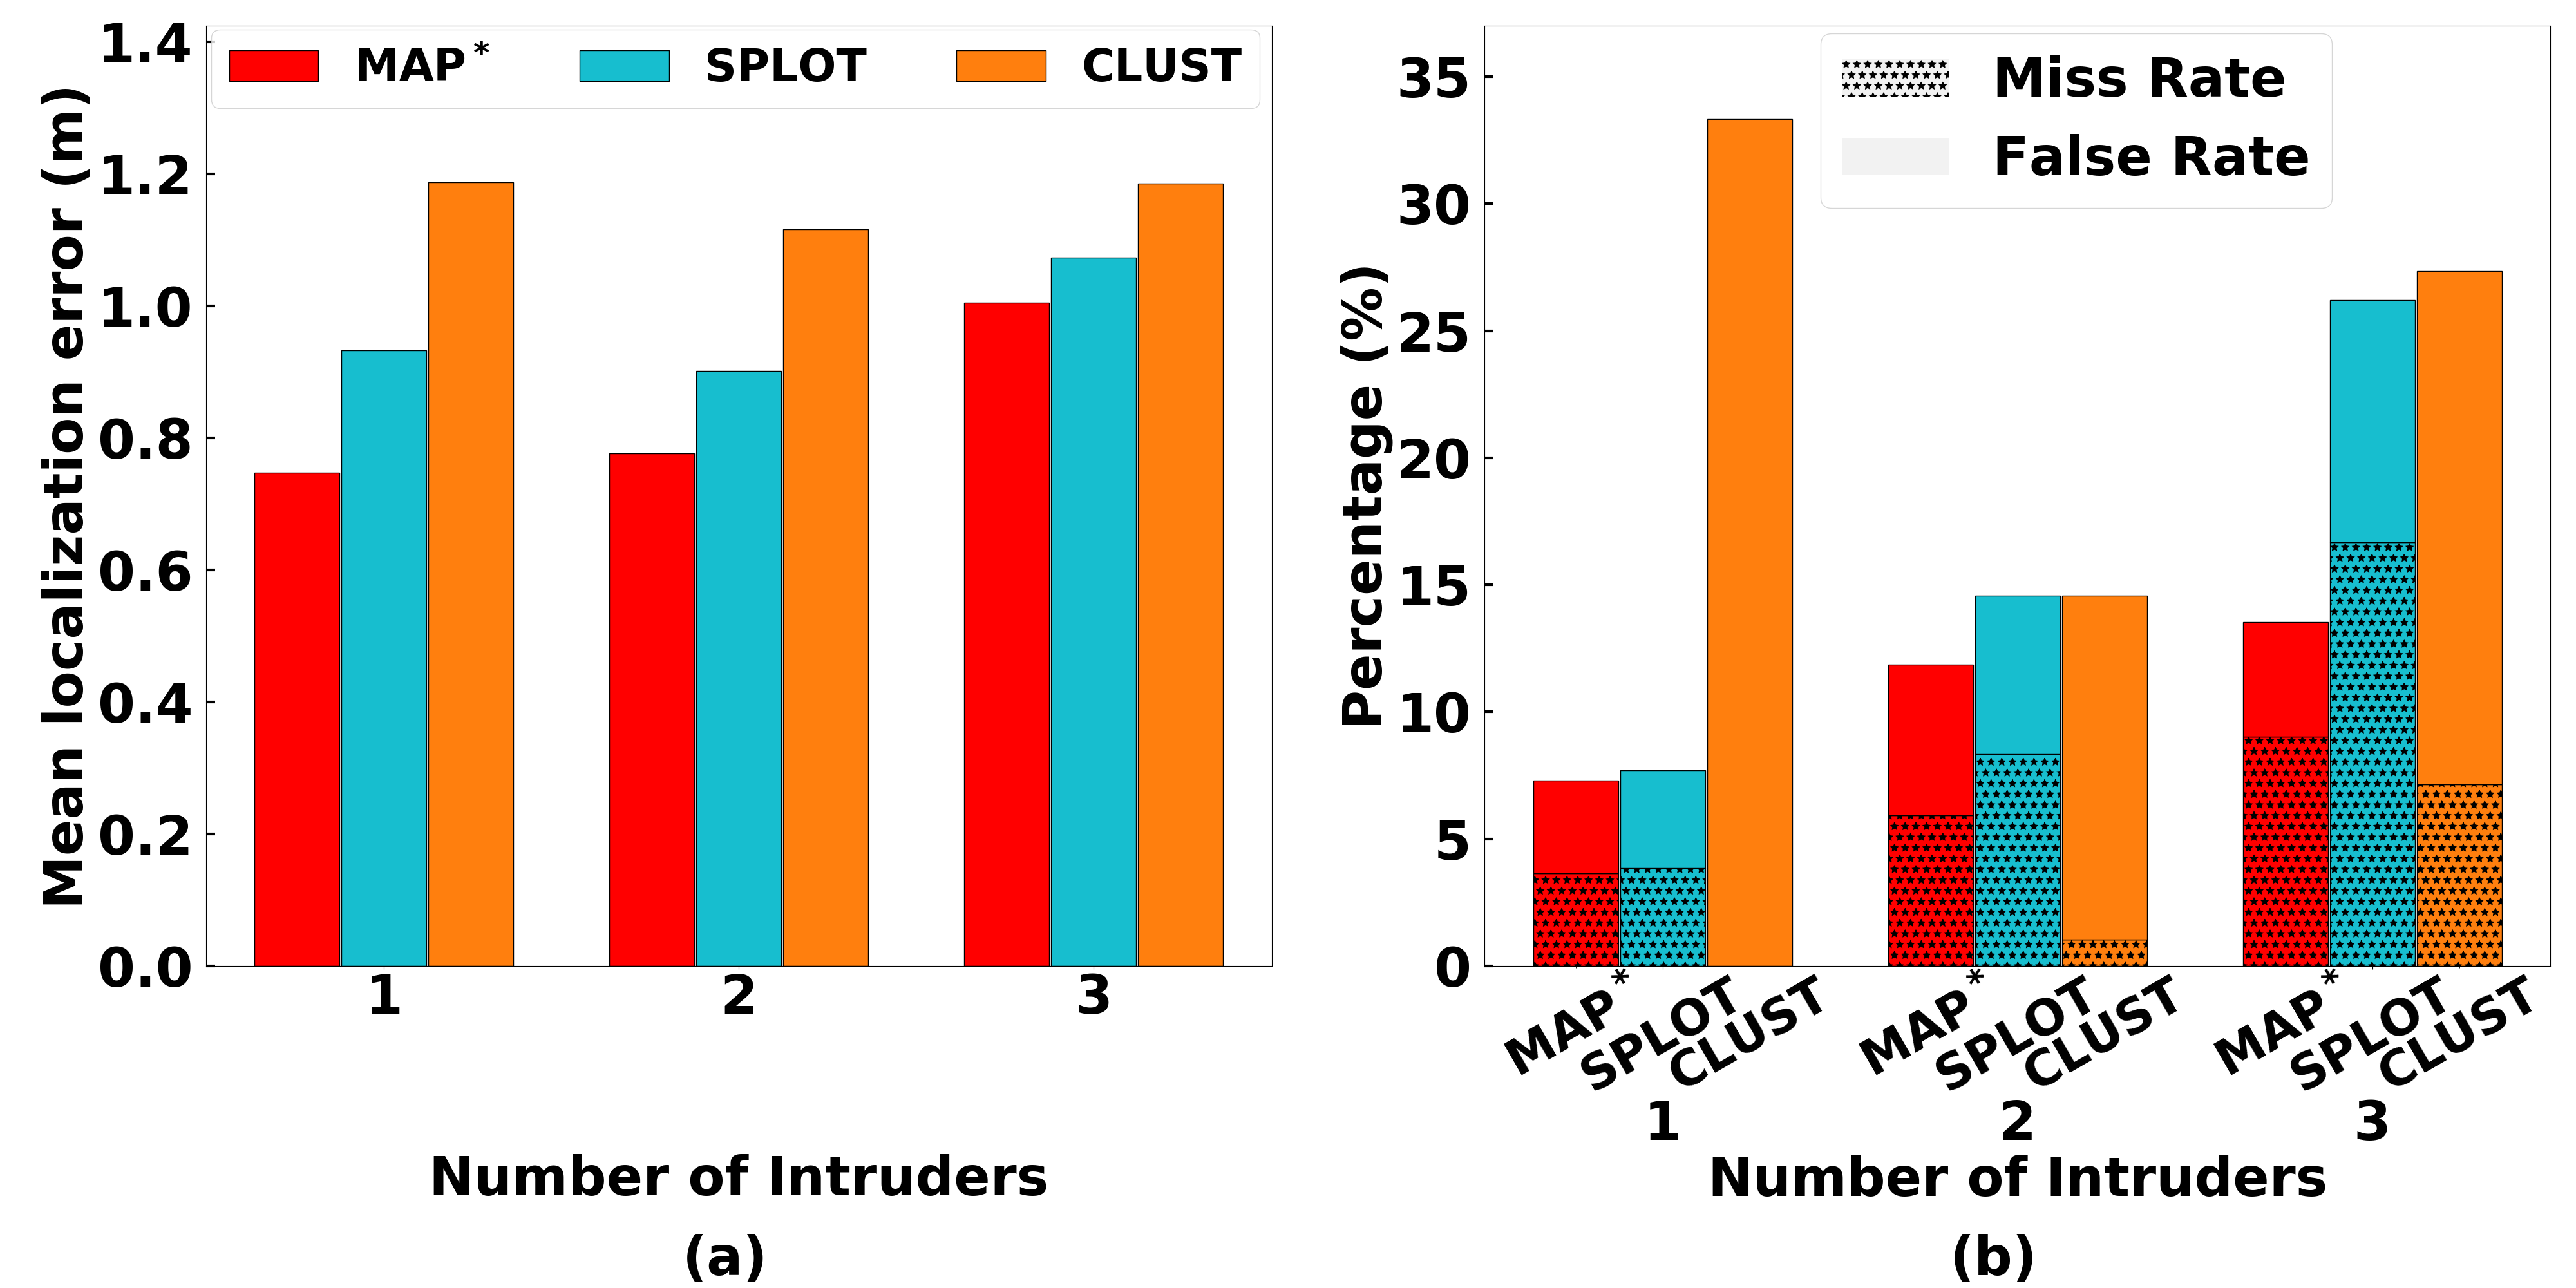
\includegraphics[width=0.8\textwidth]{chapters/ipsn/figures/indoor-error-missfalse.png}
	\caption{Localization performance of various algorithms in an indoor testbed}
	\label{fig:indoor-error-miss-false}
\end{figure}

\begin{figure}[ht]
	\centering
	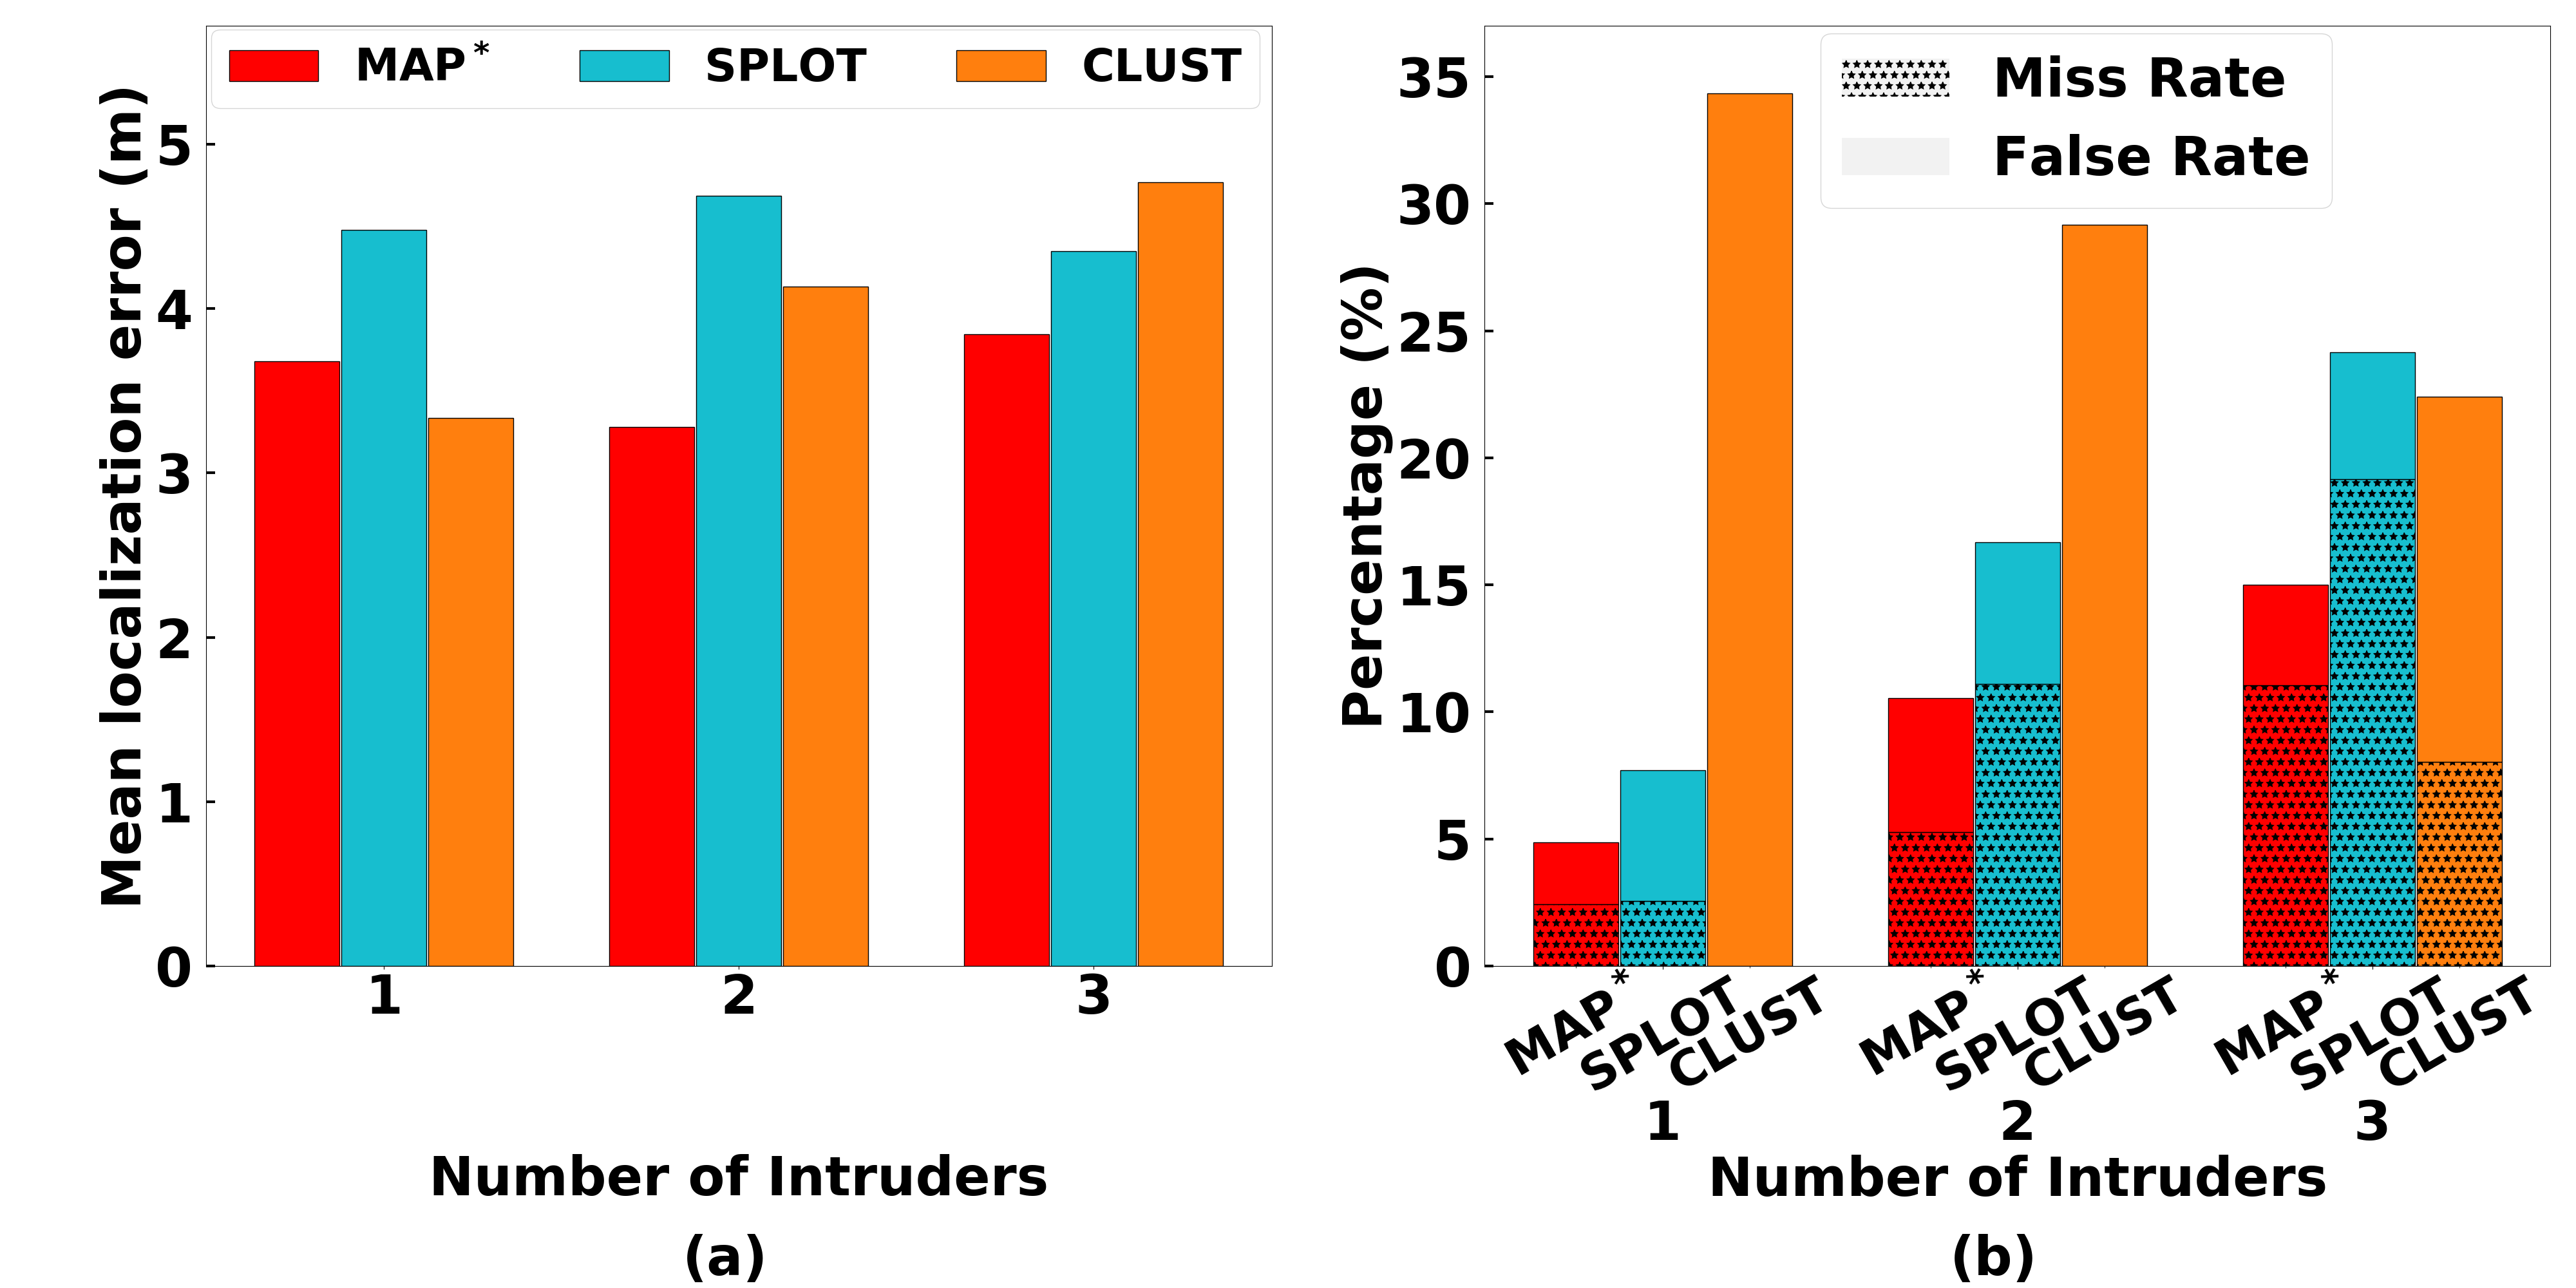
\includegraphics[width=0.8\textwidth]{chapters/ipsn/figures/outdoor-error-missfalse.png}
	\caption{Localization performance of various algorithms in an outdoor testbed}
	\label{fig:outdoor-error-miss-false}
\end{figure}

\para{Evaluation.}  For evaluation, in both testbeds, we place the 18
sensors at centers of grid cells that are randomly chosen and are
different from the cells chosen for the training above. The chosen
locations for the outdoor testbed are shown in
Fig.~\ref{fig:outdoor}(b). We choose the intruder's gain/power to be
in the range of [$\pstar-1, \pstar+1$], where $\pstar$ is the
gain/power used during the training phase as mentioned above.
%%%%%
Roughly half of our experiments involve close-by (in the same or
adjacent grid cells) intruders. Localization is done on a laptop which
listens to HTTP requests containing the sensors' observations. 

\subsection{Results}




\para{Localization Metrics.}
Figure~\ref{fig:indoor-error-miss-false}-\ref{fig:outdoor-error-miss-false}
show the localization results for the indoor and outdoor testbeds
respectively. Overall, the results indicate that \ouralgo performs the
best across all metrics, with the overall performance gap between
\ouralgo and \splot increasing with the increase in number of
intruders. When the number of intruders is 3, the performance of
\splot is significantly worse than \ouralgo due to a
significantly higher (84\% for indoors and 53\% for outdoors) sum of miss and false-alarm rates and 43\% higher localization error.
%%%%
The \cl algorithm generally performs the worst, but its
performance doesn't have a strong correlation with the increase in the
number of intruders; recall that \cl is given the range of number of
intruders as an extra piece of information compared to the other
algorithms.  In terms of absolute performance, we see that the
localization error of \ouralgo is roughly around 1 or less grid cell,
and the sum of miss-rate and false-alarm is between 5-15\%.


\begin{table}[ht]
	\centering
	\caption{Interpolation Mean Absolute Error (MAE) and  Mean Error (ME) in dB for \idw and \ildw}
	\begin{tabular}{c | c c c c}
		\hline\hline
		& \idw & \ildw &  \idw & \ildw \\ 
		Environment & (MAE) & (MAE)  & (ME) &  (ME) \\
		\hline 
		Indoor &  2.6 & 1.7  &  1.7 & 0.25  \\
		Outdoor & 6.2 & 2.7 & 5.8 & 0.48  \\
		\hline %inserts single line
	\end{tabular}
	\label{tab:inter-error}	
\end{table}



\para{Interpolation Error.}
Table \ref{tab:inter-error} shows the
interpolation mean absolute error (MEA) as well as mean error (ME) of
\idw and \ildw when the transmitter and receiver are close by (i.e.,
within a distance of 3 grid cells). When the transmitter and receiver
are far away, the difference between \idw and \ildw is small and thus not
shown.  We see that when compared with \idw, our \ildw interpolation
scheme decreased the mean absolute error by 35 percent in the indoor
environment and 56 percent in the outdoor environment.  In terms of
mean error, \ildw reduced the error compared to \idw by as large as 86
percent and 92 percent respectively. This is because \idw
mostly tends to estimate the value to be larger than the ground truth,
while \ildw's estimates are more even across the ground truth.

\begin{table}[ht]
	\caption{Power Prediction Mean Absolute Error (MAE) and Mean Error (ME) in dB for indoor and outdoor testbed}
	\centering
	\begin{tabular}{c | c c c c}
		\hline\hline
		& Indoor & Outdoor & Indoor  & Outdoor  \\
		\# Intruder  & (MAE)   &    (MAE)   &  (ME)  &   (ME)     \\
		\hline
		1 & 0.34 & 0.50 & -0.02 &  0.02 \\ 
		2 & 0.57 & 0.63  &  0.10 & 0.54\\
		3 & 0.77 & 0.90 & 0.49 & 0.76\\
		\hline %inserts single line
	\end{tabular}
	\label{table:power-error}
\end{table}

\para{Intruder Power.}  Table ~\ref{table:power-error} shows the errors in the predicted powers of
the intruders in \ouralgo. We see that the outdoors have a slightly
higher power prediction error, likely because of a larger number of
grid cells. We also note that with the increase in the number of
intruders, the error in predicted power increases.






\section{conclusions}

In this paper, we have developed an efficient Bayesian approach with a noval interpolation scheme to
localize multiple transmitters in presence of authorized users, and
demonstrate its superior power over large-scale simulations and smaller
scale indoor and outdoor testbeds.
%%%%%%
In our future work, we wish to extend our techniques to allow a
continuous location domain and design methods to further minimize
training cost. In addition, we will consider alternate signal
measurements such as angle-of-arrival (AoA).





\section*{Acknowledgments}

The work is supported by NSF grants CNS-1642965 and CNS-1815306. 
Thanks to Salman Qavi and Jayesh Ranjan for their help during the testbed.
Also thanks to Samir Das, Petar Djuric and Peter Milder for providing advice during group meetings.



